\documentclass[11pt]{book}
\usepackage{classicthesis}

%\documentclass[10pt]{llncs}
%\usepackage{llncsdoc}
% \usepackage[sc,osf]{mathpazo}   % With old-style figures and real smallcaps.
% \linespread{1.025}              % Palatino leads a little more leading
% % Euler for math and numbers
% \usepackage[euler-digits,small]{eulervm}
\usepackage{bbding} % for flower. 
\usepackage{physics}
\usepackage{amsmath,amssymb}
\usepackage{graphicx}
\usepackage{makeidx}
\usepackage{algpseudocode}
\usepackage{algorithm}
\usepackage{listing}
\usepackage{minted}
\usepackage{cancel}
\usepackage{quiver}
% \evensidemargin=0.20in
% \oddsidemargin=0.20in
% \topmargin=0.2in
%\headheight=0.0in
%\headsep=0.0in
%\setlength{\parskip}{0mm}
%\setlength{\parindent}{4mm}
% \setlength{\textwidth}{6.4in}
% \setlength{\textheight}{8.5in}
%\leftmargin -2in
%\setlength{\rightmargin}{-2in}
%\usepackage{epsf}
%\usepackage{url}

\usepackage{booktabs}   %% For formal tables:
                        %% http://ctan.org/pkg/booktabs
\usepackage{subcaption} %% For complex figures with subfigures/subcaptions
                        %% http://ctan.org/pkg/subcaption
\usepackage{enumitem}
%\usepackage{minted}
%\newminted{fortran}{fontsize=\footnotesize}

\usepackage{xargs}
\usepackage[colorinlistoftodos,prependcaption,textsize=tiny]{todonotes}

\usepackage{hyperref}
\hypersetup{
    colorlinks,
    citecolor=blue,
    filecolor=blue,
    linkcolor=blue,
    urlcolor=blue
}

\usepackage{epsfig}
\usepackage{tabularx}
\usepackage{latexsym}
\newcommand\ddfrac[2]{\frac{\displaystyle #1}{\displaystyle #2}}
\newcommand{\N}{\ensuremath{\mathbb{N}}}
\newcommand{\R}{\ensuremath{\mathbb R}}
\newcommand{\coT}{\ensuremath{T^*}}
\newcommand{\Lie}{\ensuremath{\mathfrak{L}}}
\newcommand{\Vectorfield}{\ensuremath{\mathfrak{X}}}
\newcommand{\pushforward}[1]{\ensuremath{{#1}_{\star}}}
\newcommand{\pullback}[1]{\ensuremath{{#1}^{\star}}}
\newcommand{\vectorfield}{\ensuremath{\mathfrak{X}}}

\newcommand{\pushfwd}[1]{\pushforward{#1}}
\newcommand{\pf}[1]{\pushfwd{#1}}

\newcommand{\boldX}{\ensuremath{\mathbf{X}}}
\newcommand{\boldY}{\ensuremath{\mathbf{Y}}}


\newcommand{\G}{\ensuremath{\mathcal{G}}}
% \newcommand{\braket}[2]{\ensuremath{\left\langle #1 \vert #2 \right\rangle}}


\def\qed{$\Box$}
\newtheorem{theorem}{Theorem}
\newtheorem{corollary}[theorem]{Corollary}
\newtheorem{definition}[theorem]{Definition}
\newtheorem{lemma}[theorem]{Lemma}
\newtheorem{observation}[theorem]{Observation}
\newtheorem{proof}[theorem]{Proof}
\newtheorem{remark}[theorem]{Remark}
\newtheorem{example}[theorem]{Example}

\newcommand{\X}{\ensuremath{\mathfrak{X}}}

\title{General Relativity and Differential Geometry}
\author{Siddharth Bhat}
\date{Monsoon 2019}

\begin{document}
\maketitle
\tableofcontents

\chapter{Special relativity}

\section{Galileo's principle of relativity}
\section{Einstein's principle of relativity}
All laws of physics are the same in all inertial frames.
Negative definition: No test allows us to differentiate
\section{Emptiness}
Is relativity just a postulate? What lies behind it? It depends on
``space is empty''. All the fields that we see are all dancers on the
stage which is empty space. Empty space cannot distinguish between anything
(isometry and isotropy of space). Space cannot make a choice between observers,
etc.

But is space really empty? No. At very big distances, we get galaxies etc. But
all of this dust is within space, not a part of the space, so it is okay. We need
to sample massive areas over massive timescales.

But once we get to QM, we know that we have virtual partices. We need to sample
very small locations for very small times. If we restrict ourselves, to not
allowing such observations, then we escape this.

But we can always choose slices of spacetime which are empty.

We have two overlapping reference frames. They are observing the same experiment,
which is separated by two events. In one frame, we get $\delta x, \delta t$. In
the other frame, we will get $\delta x', \delta t'$. So they will not
agree on velocities and forces. 

Assume we have a current carrying conductor lying in a 2D plane along the y axis.
Current is travelling from -infinity to plus infinity. The magnetic field on the
left half is outward [Biot-savart].

There is a proton in the left half plane moving parallel
to the y axis northward. It'll be attracted towards the wire.
The force is going to be $F = qv \times B$ [Lorentz force laws].

So if we are at rest, I'll see a proton that is changing the direction of its
velocity, but not the direction because the force is perpendicular to the
velocity.

Now if we are on the proton, We are originally stationary, so we then starting
travelling towards the proton. This means that we have an electric field.

Two observers will not agree on electric and magnetic field strengths either!


\section{What do two different inertial frames agree upon?}
One is the laws of physics, and fundamental constant of nature [speed of light].
They will also see the same space-time separation $t^2 - x^2$.

Is the speed of light a fundamental constant of nature? Or is it just a
conversion factor? in cartography, we have metres and miles. In spacetime,
we have seconds and metres.

The \emph{value of the speed of light} is not a fact of nature, since the value
is measured in some units. 

Better measurements of the speed of light just give us better ratios between
units of space v/s units of time.

\section{Relativity of simultaneity}

Can we say that two events happen at the same time? No, two different frames
will not agree on the simultaneity of two different events.


If two different observers cannot even agree on the $\delta x$, how will they
agree on $\delta t = 0$? Insert train paradox here.


Since two flashes struck on two sides and we are at the midpoint, the flashes
of light will reach us simultaneously. We can measure the length.


The observer in the train will argue that the lightning was not simultaneous,
since they are moving towards the light, the light ray in the front will reach
earlier than the light ray in the back.

If we disagree about simultaneity, we disagree about length.
The rest length [that is, the length of the rod when it is in rest with respect
is called proper length]. All observers will agree on the proper length.


We can look at lack of simultaneity as "time dilation", because for one,
we had $\delta t = 0$ [on the ground], while on the other, we had $\delta t > 0$,
where the $\delta t$ is the time elapsed between the two events.

We have two parllel mirrors and a pulse of light keeps going back and forth.
A unit of time is the time it takes to go from one mirror to the next. One period
has two time units.


When we talk about relativity, we are only talking about inertial. Velocities
are relative, acceleration is not. We can figure out that there is acceleration
from within a frame by doing something like jumping. So all motion is relative,
as long as we have inertial frames.


In the case of the rocket ship, We have one frame that sees acceleration while
the other does not. So that rocket ship dude knows that he has aged. The
solution to the twin paradox ought to be in GR, because one of the frames sees
acceleration while the other does not.

What happens if we use pendulums inside SR? Will we have time go faster
or whatever?

Notice that in any thought experiment of SR, we always say "we have stuff moving",
we never say that "we start moving". Because otherwise, we would have forces
(acceleration) which is not explained by SR.


Will a mechanical clock observe the same time as a light clock? Yes. Why? Let's
assume we have two light clocks, one in the rest frame and one in the moving
frame. Now the mechanical clock in the rest frame is setup to match the light
frame [by construction]. Now in the moving car, we better have the mechanical
clock match the light clock. Otherwise, we can see the difference between
two clocks.

Why doesn't thickness change? We are moving along the length of the rod, and
the thickness is perpendicular to the direction of motion. Perpendicular
implies a "single direction". "Transverse" implies an entire collection of
directions.

Let us say that with respect to me, I observed a thickness contraction.
Then in my frame, the axle of the train should be too small to fit on the track.
On the other hand, if I sit in the train, I'll see that the tracks are moving.
So I should see that the separation between the tracks should be too small
for the axle. This is a paradox, so we are forced to say that there is no change
in the transverse dimension.

Can we argue the same thing using light clocks?

There is an argument using two cylinders. Imagine two hollow cynlinders which
we cut into parts. Call the, $l$ and $r$. Since they were part of the same
pipe, they ought to collide on edge. If there was thickness contraction, the
observer assigned to the $l$ pipe will say that the observer of the $r$ pipe
will argue that the radius of the $r$ pipe is smaller than the $l$ pipe,
and vice versa.

Is there an axis of shrinkage? No, it ought to occur equally for all axes.

If we have a set of events that occur at the ring of the $l$ frame. Then they
will be simultaneous in the $r$ frame. Why? because assume not. Then which
even will occur first? Whichever you pick, you'll break isotropy of space.
The $r$ observer can detect the absolute orientation. Hence transverse
dimensions don't change, and simultaneity is invariant in the transverse
dimension. Shenanigans only happens along the direction of motion. Perpendicular
to it, two different overlapping observers will agree.


Proof of invariance of the interval.

Can we derive equations for pendulum? From 7th to 12th question are problems.
Read through all of them and figure out what I want to solve.

\chapter{Taylor Wheeler: Lorentz Transformations}

So far, our description is lacking because we can only work with events
and intervals between events. We don't know how to work with general
coordinate transforms. Up until now, we've only said that time dilation
happens and length contraction happens, but we have had no formulae for this.
Since we cannot travel faster than light, we cannot naively add velocities.
We need the spacetime interval to be invariant. The unprimed coordinates are
lab frame $(x, t)$ and a  primed are lab frame $(x', t')$.
Rocket is moving with constant velocity $v$ with respect to the lab. We have
$x' = Ax + Bt; t' = Cx + Dt$.

If $x' = f(x, t)$. We set $x' = 0$. This gives us $f(x, t) = 0$. From this
we try to calculate the velocity of the primed origin in my frame. This velocity
must be independent of $x$ and $t$. The velocity of this point with $x' = 0$
should have velocity $v$. This velocity should be constant across $x$ and $t$.

$$
dx' = (df/dx) dx + (df/dt) dt \\
dx' = 0 \text{(we are choosing $x'$ as constant.)} \\
-(df/dt)/(df/dx) = dx/dt = v \\
$$

This value ought to be independent of $x$ and $t$. Because all frames are
initial, we're fine. We can't have a dependence on $t$ since that would be
some kind of acceleration. We can't have dependence on $x$ as well, since
space is isotropic.

We can have:

$$ (df/dt) = -v (df/dx) $$
We want this to be a \emph{constant} however. We need both $df/dt$ and $df/dx$
to be constant functions. How do we show that?

$$x' = Ax + Bt; t' = Cx + Dt$$ We set $x' = 0$. This gives is $Ax + Bt = 0$,
or $x = -B/At$. Hence $-B/A = v$. So $B = -Av$. $x' = A(x - vt)$.
$x = A(x' + vt')$, by symmetry.

Set $x' = ct'$, $x = ct$, because the speed of light is invariant. We assume
that the spacetime origins coincide.


$$
x = A(ct + ct') \\
c^2 t't = A^2t' t(c^2 - v^2) \\
...
x' = 1/\sqrt{1-v^2/c^2}
$$

$$
x'/t' = x/t
$$

\section{invariance of light speed implies invariance of the interval}
$x = ct$

From which I can derive:
$$c^2t^2 - x^2 = 0$$


$x = ct$

\section{Invariance of interval implies invariance of light speed}
$$
t*t - x*x = c = t'*t' - x'*x'
$$

\section{addition of velocities}

$$
x' = \gamma(x - vt)
t' = \gamma (t - vx/c^2)
$$

$$
x'= v_b' t'
\gamma(x - vt) = v_b' \gamma(t - vx/c^2) 
(x - vt) = v_b' (t - vx/c^2) 
(c^2x - c^2 vt) = v_b' (c^2t - vx) 
(c^2 + v)x = t(v + v_b') \\
$$

We want to find out $\frac{dx}{dt}$.


\chapter{Theoretical Minimum: Introduction: Lecture 1}

I am following the lecture series of the theoretical minimum by Susskind.

A reference frame is a set of spatial co-ordinates. To specify, we will need
to specify the origin and the orientation of th co-ordinates.
[TODO: add the arnold stuff here].

If a frame is inertial, then any frame moving with constant velocity to it
is inertial. A first inertial frame is one where newton's laws are correct.
Hence, particles with no forces on them move with uniform velocity.
`F = ma` together with coloumb's law of attraction is the same in every
reference frame.

We cannot tell if we are in a moving reference frame or not.

Einstein added a law of physics: the speed of light is $c$. The principle of
relativity said that physics is the same in all reference frames. This
together gives us the fact that the speed of light is $c$ is \emph{all}
reference frames.

We start with a reference frame along the $x$ axis. we have a $t$ axis. Call
this my reference frame. Light moves at the speed of light. If a light
ray is sent out from the origin, it will move with a trajectory given
by $x = ct$. Now we will add a second reference frame with an $x'$ axis,
whose center moves relatively to the $x-t$ coordinate system. This
moves at speed $vt$. $x' = x - vt$.

Newton made the assumption that all clocks are synchronized --- that is,
$t' = t$. Let's now ask how the light ray moves in the $x'-t'$ frame.
We will get $x' = ct - vt = (c - v)t = (c - v)t'$. So for me, the
speed of light is $(c - v)$. Something is \emph{wrong!} --- the light ray
ought to move at speed $c$. We need to figure out how to change for the
speed of light to remain the same.

Experimentally, how would we synchronize clocks? observers $A, B$ can
find someone in the middle [which we can measure with our meter sticks],
call them $C$. We will check our clocks by having $A, B$ send a flash of light
to $C$ when their clocks read $12:00_{A, B}$. If the light reaches at the same
time from $A, B$ to $C$, then the clocks are synchronized.

Now, if I'm moving, I'm $D$, who is at moving from $A$ to $B$. The light
reaches $D$ at two different times for $D$. so it's unclear how to define
synchronous.


We have (Fred) $x = vt$, and $x' = 0$ on the same line. We want to figure out
where the $t'$ axis is. We have (Mary) $x = vt + 1$ . The
third person, (Seymour) is $x = vt + 2$. [all of these are relative to the stationary coords].
The moving and stationary observer agree on what $t = 0$ means. Fred will
send out a light signal to Mary. Seymour will also send out a light signal
to Mary. They send it in such a way that they arrive to mary at the same
time. The point will occur above $t = 0$ for Seymour. Let $a$ be the
time mary gets fred's light ray. Let $b$ be the "backtraced" point from
mary to fred along -45 degrees.

Point $a$ is the intersection of $x = t$ [c = 1] (Light from Fred) 
with $x = vt + 1$ (Mary). We get $t = vt + 1$, or $t = 1/(1-v)$. since
the light ray line is $x = t$, we get $x = t = 1/(1-v)$.

Next, for line $ab$: the equation is going to be $x + t = const$, since it
has slope -45 degrees. We can plug in the value of point $a$ into $x +t = const$
to discover $const$. we get $1/(1-v) + 1/(1-v) = const$, which means
$const = 2/(1-v)$. Next, we find the intersection of $ab$ ($x+t = const$)
with $x - vt = 2$.

If we subtract the two equations, we get
$t(1+v) = 2(1/(1-v) - 1) = 2[1 - (1-v)]/(1-v) = 2v/(1-v)$.
Hence, $t = 2v/(1+v)(1-v) = 2v/(1-v^2)$.

We know that $x_b = 2/(1-v) - t_b = 2/(1-v) - 2v/(1-v^2) = $
\chapter{GR: Introduction}

I am following the following sources:

\begin{itemize}
    \item Susskind's General Relativity lectures as part of the Theoretical
        minimum: (\href{https://theoreticalminimum.com/courses/general-relativity/}{The link is here}).
        Note that the videos do not load. However, one can view the source to access the link
        to the iframe.
    \item Susskind's other General Relativity lectures, as part of his modern
        physics course: (\href{https://www.youtube.com/watch?v=hbmf0bB38h0&list=PL6C8BDEEBA6BDC78D}{link to playlist here}).
        These seem to be taught at a much gentler pace.
    \item The book Gravitation by Misner, Thorne and wheeler.
\end{itemize}

The notes as scribed here are a mix from all of these sources, as well
as tangential points I find interesting.

\section{The equivalence principle}

Gravity is in some sense the same thing as acceleration. First, an elementary
derivation which formalizes the intuition of the equivalence principle.

We consider an elevator moving upward. Let its distance from the bottom be $L(t)$.

\begin{align*}
    z' = z - L(t) \quad t' = t \quad x' = x
\end{align*}


% \begin{align*}
% F = m\frac{d^2 z'}{dt^2} \\
% F = m\frac{d^2 (z - L(t))}{dt^2} \\
% F = m\frac{d^2 z}{dt^2} \text{(If \frac{d^2L(t)}{dt^2} - 0)}
% \end{align*}

if $\frac{d^2 L(t)}{dt^2} = 0$, then the force is the same in the new coordinate
system as that of the old coordinate system

\section{Galileo's theory of flat space and gravitation}
Newton's laws:
\begin{align*}
    &\vec F = m \vec a \\
    &\vec F = m \frac{d^2 x}{dt^2} \\
\end{align*}

Galileo's gravitation, under the approximation that the earth is flat:
If we pick downwards to be negative direction along the $2$ dimension, then his
equation can be written as ${F_2 = - m g}$ where $g$ is a constant.

This is special, because the force is proportional to the mass, which is not
the case of things like electromagnetism.


Combining the two equations, we get ${m \frac{d^2x}{dt^2} = - m g}$, or
${\frac{d^2x}{dt^2} = - m g}$.


That the acceleration induced by the graviational force is independent of the
mass of the object is known as the \textit{equivalence principle}. At this
stage, we can say that gravity is equivalent across all objects independent of
their mass.

Let's now consider a collection of point masses --- A diffuse cloud of
particles, and have it fall. Different particles maybe heavy, light, large,
small. However, since all of them have the same acceleration, the point cloud
looks unchanged as it falls. That is, the object will have no stresses or
strains as it falls. We can't tell by looking at our neighbours that there is a
force being exterted on us, since all our neighbours are moving along with us!
We cannot tell the difference between being in free space versus being in a
graviational field.

\section{Newton's theory of gravity}
all bodies exert equal and opposite forces on each other. Given two bodies $a$
and $b$ of masses $m$ and $M$ with distance $R$, the force on $a$ is
${F_a \equiv \frac{GmM}{R^2}} \hat{r}$. where $\hat r$ is the direction from $a$
to $b$.

Again, we can prove that the acceleration of an object $a$ does not depend on
its own mass.

Now that gravitation depends on distance, we can actually feel something if we
are in a gravitational field, since different parts of a given object will have
a different force on it, due to the varying distance from (say) the earth.

Gravitational field is defined as the force exerted on a test mass at every
point in space.

\subsubsection{Gauss' theorem}
${\int  \grad \cdot A dx dy dz  = \int A_{\bot} d\sigma}$ where $\sigma$ is the
differential unit of surface area of the surface. 

Show that the divergence of a field in 3 dimensions will lead to an inverse
square law.


\section{Geometry and curvature}

To describe a geometry, all we need is the distance between neighboring points
on a blackboard. In general, given a parametrization, we can draw a possibly
distorted grid of lines of constant corrdinate. The distance between two points
${(x, y)}$ and ${(x + dx, y+ dy)}$ will be ${ds^2 = g_{11} dx^2 + 2 g_{12} d_x d_y + g_{22} d_y^2}$.


\chapter{Opimisation on Steifel Manifolds}
We have the space $O(n) = \{ X \in \R^{n \times n} | X^T X = I \}$. To find an
element of the tangent space at the point $P \in O(n)$, we parametrize a curve
$C(t) : \R \rightarrow O(n)$, such that $c(0) = P$.  Then, we differentiate the
curve and evaluate it at $0$. That is, $\frac{dc}{dt}\vert_{t=0} \in T_P O(n)$.


We consider $C(t) : \R \rightarrow O(n)$, such that $C(0) = P$.  Since $C(t) \in
O(n)$, we can write $C(t)^T C(t) = I$.  This in index notation, is $c^{ik}(t)
c^{jk}(t) = \delta^{ij}$. Differentiating with respect to $t$, we get:

\begin{align*}
&C^T(t) C(t) = I \\
&c^{ik}(t) c^{jk}(t) = \delta^{ij} \\
&\frac{d (c^{ik}(t) c^{jk}(t))}{dt}= \frac{d(\delta^{ij})}{dt} \\
& \dot c^{ik}(t) c^{jk}(t) + c^{ik}(t) \dot c^{jk}(t) = 0 \qquad \text{(chain rule)}\\
&\dot C^T(t) C(t) + C(t)^T \dot C(t) = 0
\end{align*}

Now, we know that $C(0) = P$, and hence $\dot C(0) \in T_P O(n)$. By evaluating
the above equation at $t = 0$, we obtain the relation:

\begin{align*}
&\dot C^T(0) C(0) + C(0)^T \dot C(0) = 0 \\
&\dot C^T(0) P + P^T \dot C(0) = 0
\end{align*}

Hence, we conclude that for all $Z \in T_P O(n)$, $Z^T P + P^T Z = 0$. Indeed,
we can characterize $T_P O(n)$ this way and prove the reverse inclusion (how?),
to show that:

\begin{align*}
     T_P O(n) \equiv \{ Z \mid Z^T P + P^T Z = 0 \}
\end{align*}

However, this equation for the $Z$ is "ineffective", in that it does not tell
us how to \textit{compute} the set of $Z$s. We can only \textit{check} if a
particular $Z_0 \in_? T_P O(n)$. 

We will solve the characterization of $Z$ by first solving a slightly easier
problem: $T_I O(n)$, where $I$ is the identity matrix. 

\begin{align*}
    T_I O(n) \equiv \{ Z \mid Z^T I + I^T Z = 0 \} = \{ Z \mid Z^T = -Z \}
 \end{align*}

 We now have a complete enumeration of the \textit{tangent space at the
 identity}: We know that this consists of all skew-symmetric matrices! 

 We now wish to transport this structure of $T_I O(n)$ to an arbitrary
 $T_P O(n)$.  Here, I will let you in on a secret about the structure of
 Lie groups, which we will later prove: The vector space at $T_P O(n)$ is obtained
 by multiplying by $P$ to $T_I O(n)$. 

 In this case, it tries to inform us that:

\begin{align*}
    T_P O(n) =  \{ PZ \mid Z^T = -Z \}
\end{align*}

We distrust this assertion at first, of course, so we can plug this equation back
in the characterization of $T_P O(n)$ that we had developed and see what pops out:

\begin{align*}
     &T_P O(n) \equiv \{ X \mid X^T P + P^T X = 0 \} \\
     &\text{Let $X = PZ$ where $Z^T = -Z$, and check that they satisfy the condition $X^T P + P^T X = 0$} \\
     & (PZ)^TP + P^TPZ = Z^TP^TP + P^TPZ = Z^T I + I^T Z = -Z + Z = 0
\end{align*}

Hence, they do satisfy the condition, and we can assert that at least:
$$\{ PZ \mid Z^T = -Z \} \subseteq  \{ X \mid X^T P + P^T X = 0 \}$$.

\chapter{Matrix Lie groups}

We study the structure of Lie groups, and we prove theorems about the
structure of the tangent spaces at the identity, and how this structure
governs the behavior of the tangent spaces every else on the group.

Consider a group of matrices $(G, *:G \times G \rightarrow G, I:G)$, which is equipped
with a manifold structure, where $I$ is the identity matrix, and $*$ is 
matrix multiplication.

Now, we consider the tangent space at the identity element $T_e G$. What
we want to do is to transport the structure of the tangent space at the identity
to an arbitrary point $p \in G$. For this, we consider a manifold mapping
$f: G \rightarrow G$, such that its pushforward $df: T_X G \rightarrow T_{f(X)} G$
maps $I$ to $F(I)$. That is, we would need a map such that $f(I) = p$, such that
the pushforward pushes forward $T_I G$ to $T_f(I) G = T_p G$.

We consider the map $\left( f: G \rightarrow G; f(X) \equiv P * Xs \right)$. 
$f(I) = P * I = P$, so $f$ maps $I$ to $P$.

Next, let's consider a curve $c \in T_e G$. That is, $c: (-1, 1) \rightarrow G$, such that $c(0) = I$.
Recall that all the information about the curve $c$ that defines its directional
derivative is stored in $\frac{d~ch \circ c(t)}{dt}|_{t=0}$.

Recall that the pushfoward is defined as 
\begin{align*}
&df: T_X G \rightarrow T_{f(X)} G \\
&df: ((-1, 1) \rightarrow G) \rightarrow ((-1, 1) \rightarrow G)  \\
&df(c)(t) = \frac{d~f(c(t))}{dt}|_{t=0} \quad \text{(where $c(0) = X$)} \\
&\frac{d~f(c(t))}{dt}|_{t=0} = f'(c(t))c'(t)|_{t=0} = f'(c(0)) c'(0) = f'(X) c'(0)
\end{align*}

Hence, we would like to pick a $c$ such that $c(0) = e$,
and $\frac{d~ch \circ c(t)}{dt}|_{t=0}$ is easy to compute, where $ch: G \rightarrow \R^n$
is a chart for $G$ around the point $c(0)$.
In our case, the $ch$ is just the identity function, since matrices can naturally
be considered as elements of $\R^{m \times n}$ if the matrices of $G$ are $m \times n$
matrices. So $(ch = id)$, and  the tangents reduce to $\frac{dc(t)}{dt}|_{t=0}$.
to construct such a curve $c$, we first define the matrix exponential and use it to
define the curve $c$:

\begin{align*}
&exp: G \to G \qquad exp(Y) \equiv I + Y + \frac{Y^2}{2!} + \frac{Y^3}{3!} + \cdots + \frac{Y^n}{n!} + \cdots \\
&c: (-1, 1) \rightarrow G \qquad c(t) \equiv exp(tX) \\
&c(0) = exp(0 \cdot X) = exp(0) = I 
&\frac{dc}{dt}|_{t=0} = \frac{d exp(tX)}{dt}|_{t=0} = X exp(tX)|_{t=0} = X exp(0X)
\end{align*}

\chapter{Symplectic vector spaces}

% LINK TO LECTURES:
% Symplectic geometry & classical mechanics, Tobias Osborne.
% videos link: https://www.youtube.com/watch?v=GdXyNYUD4cE

Let $V$ be a $m$-dimensional real vector space. Let $\Omega: V \times V \rightarrow V$
be a bilinear form on $V$ that is skew-symmetric:
$\forall a, b \in V, \Omega(a, b) = -\Omega(b, a)$.

\begin{theorem}
    Let $\Omega$ be a bilinear skew-symmetric map on $V$. Then there is a basis
    $u_1, u_2, \dots u_k$, $e_1, e_2, \dots e_n$, $f_1, f_2 \dots f_n$ such that:
    \begin{itemize}
        \item $\Omega(u_i, v) = 0 \quad \forall v \in V$
        \item $\Omega(e_i, e_j) =  \Omega(f_i, f_j) 0$
        \item $\Omega(e_i, f_j) = \delta_{ij}$
    \end{itemize}
\end{theorem}
\begin{proof}
    Generalize Gram-Schmidt process.
    Let $U = \{ u \in V | \Omega(u, v) = 0, ~\forall v \in V \}$
    $U$ is a subspace of $V$. Let $u_1, u_2, \dots u_k$ be a basis of $U$.

    Establish $e_j, f_j$ by induction. Let $V = U \oplus W$. Take $e_1 \in W$.
    Then, there must exist an $f_1 \in W$ such that $\Omega(e_1, f_1) \neq 0$. 
    Otherwise, we could expand the size of $U$ by adding $e_1$ to $U$. But
    we assumed that $U$ contains all such vectors. $U$ and $W$ share no non-zero
    vectors since $V = U \oplus W$.  Define $W_1 \equiv span(e_1, f_1)$.  
    Now build $W_1^\Omega \equiv \{ w \in W | \Omega(w, W_1) = 0 \}$.

    We need the folloing facts:
    \begin{itemize}
        \item $W_1^\Omega \cap W_1 = \{ 0 \}$
        \item $W = W \oplus W_1^\Omega$
    \end{itemize}

    So, recurse on $W_1$.

    Finally, $V = U \oplus W_1 \oplus W_1 \cdots \oplus W_n$.
\end{proof}

\begin{remark}
    $dim(U) = k$ is invariant for $(V, \Omega)$ since $U$ was defined in a
    coordinate free way. But, remember that $k + 2n = m$, and hence $n$
    is an invariant of $(V, \Omega)$. $n$ is called as the \emph{rank} of
    $\Omega$.
\end{remark}

$\Omega$ written in the basis of $\{ u_i, e_i, f_i\}$ gives 
$\Omega = \begin{bmatrix} 0 & 0 & 0 \\ 0 & 0 & I \\ 0 & -I & 0 \end{bmatrix}$

\subsection{Symplectic maps}

Let $V$ be an $m$ dimensional real vector space over \R. Let $\Omega: V \times V \rightarrow \mathbb{R}$
be a skew-symmetric bilinear map. We define 
$\tilde \Omega: V \rightarrow V^*$, $\tilde \Omega(v)(u) \equiv \Omega(v, u)$. 
The problem is that this map has a non-trivial kernel $U = \{ u_i \}$ in general,
so we cannot use it like a metric to identify the two spaces.

\begin{definition} A skew-symmetric bilinear map $\Omega: V \times V \rightarrow \R$ is Symplectic iff
    $\tilde \Omega$ is bijective. ie, $U = \{ 0\}$. $(V, \Omega)$ is then
    called a Symplectic vector space.
\end{definition}

\section{Properties of a Symplectic map}
\begin{itemize}
    \item $\tilde \Omega$ is an identification between $V$ and $V^*$.
    \item Since each $(e_i, f_i)$ come in pairs, the dimension of the vector space $V$ is divisible by $2$. ie, $m = 2n$.
    \item We have a basis $(e_i, f_i)$ called the Symplectic basis for $V$.
    \item $\Omega$ in matrix form with respect to the Symplectic basis is $\Omega = \begin{bmatrix} 0 & I \\ -I & 0 \end{bmatrix}$
\end{itemize}

\subsection{Subspaces of a Symplectic vector space}

\begin{definition}
    A subspace $W$ of $V$ is a Symplectic subspace if $\Omega|_W$ is non-degenrate.
    For example, take the subspace $span(e_1, f_1)$.
\end{definition}


\begin{definition}
    A subspace $W$ of $V$ is an Isotropic subspace if $\Omega|_W = 0$.
    For example, take the subspace $span(e_1, e_2)$.
\end{definition}

\subsection{Morphisms: Symplectomorphism}
\begin{definition}
    A map between $(V, \Omega)$ and $(V', \Omega')$ is a linear isomorphism
    $\phi: V \rightarrow V'$ such that $\phi^* \Omega' = \Omega$. That is,
    $\Omega'(\phi(v), \phi(w)) = \Omega(v, w)$. ($\phi^*$ is the pullback).
    The map $\phi$ is called a Symplectomorphism and the spaces $(V, \Omega)$ and $(V', \Omega')$
    are said to be Symplectomorphic
\end{definition}

(Question: why do we need to define this in terms of a pullback? Why not
pushforward? ie, $\Omega(v, w) = \Omega'(\phi(v), \phi(w))$?

\subsection{Prototypical example of Symplectic space}
Let $V = \R^{2n}$. Let $e_j = (0_1, \dots, 1_j, \dots 0_n; 0_{n+1} \dots 0_{2n})$.
Let $f_j = (0_1, \dots 0_n; 0_{n+1}, \dots 1_{n+j}, \dots 0_{2n})$.
take $\{e_j, f_j\}$  as a basis for $V$.
$\Omega_0 = \begin{bmatrix} 0 & I \\ -I & 0 \end{bmatrix}$

Let $\phi: V \rightarrow V$ be a Symplectomorphism of $V$. Then, we can 
show that $M_\phi^T \Omega_0 M_\phi = \Omega_0$. ($M_\phi$ is the matrix of $\phi$
associated to the $\{e_j, f_k\}$ basis). 

\subsection{Symplectic Manifolds}
We are generalizing our symplectic vector space. We are postulating a space
that locally looks like a symplectic vector space.

Let $\omega: T_p M \times T_p M \rightarrow \mathbb R$ be a 2-form on a manifold.
This is bilinear and skew-symmetric (by definition of begin a differential form).

We say that $\omega$ is closed iff $d\omega = 0$.

\begin{definition}
    The two form $\omega$ is a symplectic form if it is closed and $\omega_p$
    is symplectic for all $p \in M$. That is, we need $\omega_p$.
\end{definition}

\begin{definition}
    A symplectic manifold is a pair $(M, \omega)$ where $\omega$ is a symplectic
    form on $M$.
\end{definition}

\subsection{Prototypical example of Symplectic manifold}
Let $M = \R^{2n}$ with coordinates $X_1, \dots X_n, Y_1, \dots Y_n$.
$\omega = \sum_i dx_i  \wedge dy_i$.  $\omega$ is symplectic since it
has constant coefficients for each $dx_i \wedge dy_i$.

Symplectic basis for the tangent space 
$T_p \R^{2n} \equiv \{ \partial_{X_i}, \partial_{Y_i} \}$.

\subsection{2 sphere as a symplectic manifold}
Let $M = S^2$ as an embedded manifold in $\R^3$.
$S^2 \equiv \{ v \in \R^3, |v| = 1 \}$.
$T_p S^2 \equiv \{ w \in R^3 | p \cdot w = 0 \}$.
This works because $p$ is normal to the plane spanned by $T_p S^2$.
We define $\omega_p(u, v) \equiv p \cdot (u \times v)$. Clearly, this is
a 2-form since it is bilinear and anti-symmetric. $\omega$ is also closed,
since there cannot be any degree 3 forms on a 2D manifold! Hence, $d\omega = 0$.

We need to check that it is non-degenrate. For any point $p \in S^2$, 
$v \in T_p S^2$, we can take $u = p \times v$. Now, $\omega_p(u, v) = p \cdot(u \times v)$ will be
a non-degenrate area of a parallelopiped. The parallelopiped is non-degenrate 
as $v, p$ are perpendicular by definition. $u$ is perpendicular to both $v$
and $p$ by construction (cross-product). (TODO: draw picture).

\subsection{Mapping between Symplectic Manifolds}
Let $(M, \Omega)$ and $(M', \Omega')$ are Symplectomorphic if $\phi: M \rightarrow M'$
is diffeomorphic, and such that $\phi^* \Omega' = \Omega$.


\subsection{Symplectic manifolds are locally like $\R^{2n}$}
\begin{theorem} (Darboux): Let $(M, \omega)$ be a $2n$ dimensional symplectic
    manifold. Let $p \in M$. Then, there is a coordinate chart called 
    as the Darboux chart $U$ with basis $X_1, \dots X_n, Y_1 \dots Y_n$ such that
    the two-form $\omega = \sum_i dx_i \wedge dy_i$.
\end{theorem}

% Lecture 9: https://www.youtube.com/watch?v=hAX7ZCMM2kQ
\section{The cotangent bundle and Symplectic forms}

Let $X$ be an n-dimensional manifold. Let $M \equiv T^*X$ be its cotangent
bundle.  $M$ is also a manifold.

Define coordinate charts on $M$, $(T^*U: X_1, X_2, \dots X_n, \xi_1, \xi_2, \dots \xi_n)$,
where $U$ is a chart on $X$, $X_1, \dots X_n$ are coordinate functions for $U$,
and $\xi_1, \dots xi_n$ are coordinates for $T^*X_{x_0}$ where $x_0 \in X$, defined
by $\xi_{x_0} = \sum_i \xi_i {dx_i}_{x_0}$.

We need to show that the transition functions are smooth.

Let $p \in U \cap U'$. We need to express coordinates in one chart
as a smooth function of coordinates in another chart. $(U, X_1, \dots X_n)$
, $(U', X_1', \dots, X_n')$ are coordinates, and let $\xi \in T_p^* M$.
$(p, \xi) \in T^*X \equiv M$.


\begin{align*}
    \xi = \sum_i \xi_i dx_i = \sum_{i, k} \xi_i \frac{\partial x_i}{\partial x'_k} dx'_k = \sum_k \xi'_k dx'_k
\end{align*}

where the $\xi'_k = \xi_i \frac{\partial x_i}{\partial x'_k}$ are smooth since
the $\xi_i$ are smooth, and that the transition maps derivaties are smooth
since the charts are smooth.

\subsection{Canonical Symplectic structure of contangent bundle}

The physicist intuition for the following is that when we consider
a particle moving on a manifold $X$. To fully specify the state of the
particle, we need both position of the particle $x \in X$, and also
momentum $p \in T^*X$ (why does it belong to contangent bundle? Intuition:
given a velocity, it returns the momentum along it??? We can also supposedly
look at how momentum transforms).
This data is called "phase space" by physicists. Mathematically, this
is the cotangent bundle.

Now, we will see the canonical symplectic structure on the cotangent bundle.
\subsection{Tautological and Canonical forms}
Let $(U, x_1, \dots x_n)$ be a coordinate chart of $X$ and 
$(T^*U, x_1, \dots x_n, \xi_1, \dots \xi_n)$ 
be the corresponding chart of $M \equiv T^*X$. We will now define a 2-form
on $M$ on the chart $T^*U$ via:
\begin{align*}
    w = \sum_j dx_j \wedge d\xi_j
\end{align*}

\begin{theorem}
     This definition is coordinate independent
 \end{theorem}
 \begin{proof}
     Consider a one-form on $T^*U \subset M$. Let $\alpha = \sum_j \xi_j dx_j$ 
     This is called as the \emph{tautological form}.
     $\alpha$ is a one-form on $M \equiv T^*X$, when $T^*X$ is treated as a manifold.
     This is also a point on $T^* X$.
     Note that $d \alpha = - \omega$. But $\alpha$ is intrinsically defined.
     $\alpha =  \sum_j \xi_j dx_j = \sum_j \xi'_j dx'_j$.

     TODO: I don't understand why this gives us coordinate independence.
 \end{proof}

\subsubsection{Coordinate-free definition}

Let $M \equiv T^* X$. There is a canonical map $\pi: M \rightarrow X$, 
$\pi(x, \xi) = x$. We are going to pullback $T^* X$ along $T^* M = T^* (T^* X)$
$(d\pi)^*: T^*X \rightarrow T^*M$.
Let $p \in M; p = (x, \xi)$. $\xi \in T_x^* X$.
We define $\alpha$ pointwise. $\forall p \in M, \alpha_p \equiv  d\pi_p^* \xi_{\pi(p)}$.
Equivalently, let $v_p \in T_p M \equiv T_p (T^*X)$. Now, $\alpha_p (v_p) \equiv \xi( d\pi_p (v_p))$.

TODO: draw example (https://www.youtube.com/watch?v=hAX7ZCMM2kQ, 43:52)

\subsubsection{Example 1}
Let $X = \R$. Now, $M = \R \times \R$. $(x, y) \in M$ (position-momentum).
$\pi: M \rightarrow X; \pi((x, y)) = x$.

\begin{align*}
&\alpha_{(x, y)} \equiv y dx 
\qquad \omega = -d\alpha = - (\partial_y y \cdot dy \wedge dx) = dx \wedge dy \\
&\alpha_{(x, y)}(v_x, v_y) = y dx (v_x \partial_x + v_y \partial_y) = y v_x
\end{align*}


\subsubsection{Example 1}
Let $X = S^1$. Now, $M = S^1 \times \R$. $(x, y) \in M$ (position-momentum).
$\pi: M \rightarrow X; \pi((\theta, v)) = \theta$.

\begin{align*}
&\alpha_{(x, y)} \equiv y d\theta \\
&\omega_{(x, y)} \equiv d\theta \wedge dy
\end{align*}

\subsection{Naturality of Tautological form}
Let $X_1, X_2$ be n-dimensional manifolds with $T^* X_1$ and $T^* X_2$ as cotangent
bundles. Let $f: X_1 \rightarrow X_2$ is a diffeomorphism. We will show that
the tautological manifolds also match.

We show that there is a diffeomorphism $f_{\sharp}: T^*X_1 \rightarrow T^* X_2$
which lifts $f$. ie, if $f_{\sharp}((x, \xi)) = (x', \xi')$, where $x' = f(x)$,
$\xi = df^* \xi'$.

\begin{theorem} The lift $f_\sharp$ of $f: X_1 \rightarrow X_2$ pulls the
tautological form on $M_2 \equiv \coT X_2$ onto the tautological form on
$M_1 \equiv \coT X_1$.
\end{theorem}
\begin{proof}
Pointwise, we wish to show that $(df_\sharp^\star)_{p_1} (\alpha_2)_{p_2} = (\alpha_1)_{p_1}$
where $p_2 = f^\sharp p_1$.

$p_2 = f^\sharp p_1 \implies p2 = (x_2, \xi_2), x_2 = f(x_1) \land df^\star(\xi_1) = \xi_2$.

TODO!
\end{proof}

\chapter{Vector fields and flows}
% Lecture 10: https://www.youtube.com/watch?v=kGZQJALLFiE&list=PLDfPUNusx1EoVnrQcCRishydtNBYU6A0c&index=10

TODO: integrate with notes on computer

\begin{theorem}
    For any point $x \in M$, there exists a differentiable function $\sigma: \R \times M \rightarrow M$
    such that $\sigma(0, x) = x$, $\sigma(t, \sigma(s, x)) = \sigma(t + s, x)$,
    and the map $t \mapsto \sigma(t, x)$ satisfies nice properties (which ones?)
\end{theorem}
\begin{proof}
\end{proof}

\begin{definition}
    Let $\sigma: \R \times M \rightarrow M$ be a flow. Write $\sigma_t(p) \equiv \sigma(t, p)$.
    The map $\sigma_t$ is an \textbf{isotopy} if each $\sigma_t: M \rightarrow M$
    is a diffeomorphism and $\sigma_0 \equiv \text{identity}$.


    Conversely,  on a \emph{compact} manifold $M$, there is a one-to-one correspondence
    between isotopies and time-dependent vector fields, given by the equation:
    \begin{align*}
        (\partial_x \sigma_t)(x_0) = v_t(\sigma_t(x_0))
    \end{align*}
\end{definition}

Note that the situation can get complicated even on compact manifolds. Eg. a
vector field on a torus with constant irrational slope --- The space foliates
with 1D subspaces. (TODO: add picture)


\begin{definition}
    When $X = v_t$ is independent of $t$, the isotopy is said to be the
    \textbf{exponential map of the flow of $X$}. It is denoted by
    $\sigma^\mu(t, x) \equiv exp(tX) x^\mu$.
    $\{ exp(tX): M \rightarrow M \mid t \in \R \}$ is a unique,
    smooth family of diffeomorphisms, satisfying:
    \begin{itemize}
        \item $exp(0X) = id$
        \item $\partial_t exp(tX) = X \circ exp(tX)$
    \end{itemize}
\end{definition}

Let us justify naming this object $exp$:
\begin{align*}
    &\sigma^\mu(0 + t, x) = \text{taylor series around $t = 0$} \\
    &\quad = x^\mu + t (\partial_t \sigma^\mu)(0, x) + \frac{t^2}{2!} (\partial_t \partial_t \sigma^\mu)(0, x) + \dots \\
    &\quad = e^{t \partial_t} \sigma^\mu(t, x) |_{t=0} = e^{t X} \sigma^\mu(0, x)
\end{align*}

\begin{definition}
    The flow $\sigma_t$ satisfies:
    \begin{itemize}
        \item $\sigma(0, x) = exp(0X)$
        \item $\partial_t \sigma(t, x) = X(e^{tX}(x))$
        \item $\sigma(t, \sigma(s, x)) = \sigma(t, e^{sX} x) = e^{tX} (e^{sX} x) = e^{(t+s)X} x = \sigma(t + s, x)$
    \end{itemize}
\end{definition}

\chapter{Lie derivatives}
\section{The definition of the lie derivative}
The problem with manifolds is that to compare values at $x, y \in M$, it's
unclear how to compare objects. We simply cannot, since there is no structure
available to do this. So, we construct the lie derivative. Given two vector
fields $X, Y$. Let $\sigma(s, x)$ and $\tau(t, x)$ be the flows generated
by $X, Y$ respectively. Hence, $(\partial_s \sigma^\mu)|_{(s, p)} = X(\sigma(s, p))$,
$(\partial_t \tau^\mu)|_{(t, p)} = X(\tau(t, p))$.

The derivative of $Y$ along the integral curve $\sigma$ generated by $X$ is:
\begin{itemize}
    \item map $Y(\sigma_\epsilon(x)): T_{\sigma_\epsilon(x)}$ to $T_x M$,
    by $\pf{\sigma_{-\epsilon}}: T_{\sigma_{\epsilon}(x)}M \rightarrow T_x M$.
    \item Take the difference at $x$, between $(\pf{\sigma_{-\epsilon}}(Y(\sigma_\epsilon(x)))$ and $Y(x)$.
    \item Let $\epsilon \to 0$: 
        $\Lie_X Y \equiv \lim_{\epsilon \to 0} \frac{1}{\epsilon} \pushforward{\sigma_{-\epsilon}}(Y(\sigma_\epsilon(x))) - Y(x)$.
\end{itemize}

\section{Coordinate definition of Lie derivative}

Let $(U, \phi)$ be a chart with coordinates $X^\mu$. We define $e_\mu \equiv \partial_{X_\mu}$ We write
all our objects in terms of this chart.

\begin{itemize}
\item $\mathbf{X} \equiv \mathbf{X}^\mu e_\mu$
\item $\mathbf{Y} \equiv \mathbf{Y}^\mu e_\mu$
\item $\sigma_{\epsilon}^i(x) = x^i + \epsilon \mathbf{X}^i$
\item $\sigma_{-\epsilon}^i(x) = x^i - \epsilon \mathbf{X}^i$
\item $\mathbf Y^j(\sigma_\epsilon(x)) = 
    \mathbf Y^j(x + \epsilon \mathbf X) = 
    Y^j + \epsilon \mathbf X^k \partial_k \mathbf Y^j$
\item $\sigma_{-\epsilon~\star}^i(v) =
        v^j \partial_j \sigma_{-\epsilon}^i = 
        v^j \partial_j (x^i - \epsilon \mathbf X^i) =
        v^j (\delta^i_j - \epsilon \partial_j\mathbf X^i)$
\item $\sigma_{-\epsilon~\star}^i(Y(\sigma_\epsilon(x)) = 
    \mathbf Y(\sigma_{\epsilon}(x))^j (\delta^i_j - \epsilon \partial_j\mathbf X^i) =
    (\mathbf Y^j + \epsilon \mathbf X^k \partial_k \mathbf Y^j) (\delta^i_j - \epsilon \partial_j\mathbf X^i)
    = \mathbf Y^j \delta_j^i + \epsilon(\mathbf X^k \partial_k \mathbf Y^j \delta_j^i 
    - \mathbf Y^j \partial_j \mathbf X^i) + \epsilon^2(\dots)
    = \mathbf Y^i + \epsilon(\mathbf X^k \partial_k \mathbf Y^i - \mathbf Y^k \partial_k \mathbf X^i)
    $

\item $(\lim_{\epsilon \to 0} \frac{1}{\epsilon} \pushforward{\sigma_{-\epsilon}}(Y(\sigma_\epsilon(x))) - Y(x))^i =
    \frac{1}{\epsilon}(\mathbf Y^i + \epsilon(\mathbf X^k \partial_k \mathbf Y^i - \mathbf Y^k \partial_k \mathbf X^i) - Y^i)
            = \mathbf X^k \partial_k \mathbf Y^i - \mathbf Y^k \partial_k \mathbf X^i$
\end{itemize}

\begin{example}
Manifold $M$, chart $\phi$, coordinates $X^1, X^2$.
$P \equiv  -X^2 \partial_{X^1} + X^1 \partial_{X^2}, Q \equiv (X^1)^2 \partial_{X^1} + X^2 \partial_{X^2}$. The lie derivative
is computed as:
\begin{align*}
\Lie_X Y &= \{ (-X^2 \partial_{X^1} + X^1 \partial_{X^2})(X^1)^2 - ((X^1)^2 \partial_{X^1} + X^2 \partial_{X^2})(-X^2) \} e_1 + (\dots)e_2 \\
&\quad = \{ (-X^2 (2X^1) + 0) - (0 + X^2 (-1)) \} e_1 + (\dots e_2)
\end{align*}
\end{example}

\subsection{The lie bracket}
\begin{definition}
Let $X^\mu \partial_\mu, Y^\mu \partial_\mu \in \mathfrak{X}(M)$. We define
the lie derivative as $[X, Y] \equiv [X, Y](f) = X(Y(f)) - Y(X(f))$. 
\end{definition}
Now this
might have second-order derivatives. However, for it to be a vector field,
it is only allowed to have first order derivatives. 
Let's prove that the lie bracket only contains first-order derivatives.

\begin{align*}
&[X, Y]f 
    = \sum_{\mu, \nu} X^\mu \partial_\mu (Y^\nu \partial_\nu f) - Y^\mu \partial_\mu (X^\nu \partial_\nu f)
\\ &\quad = \sum_{\mu, \nu} X^\mu (Y^\nu \partial_\mu \partial_\nu f + \partial_\nu f \partial_\mu Y^\nu)
         - Y^\mu (X^\nu \partial_\mu \partial_\nu f + \partial_\nu f \partial_\mu X^\nu)
%
\\ &\quad = (X^\mu Y^\nu \partial_\mu \partial_\nu f - Y^\mu X^\nu \partial_\mu \partial_\nu f + 
    \partial_\nu f (X^\mu \partial_\mu Y^\nu - Y^\mu  \partial_\mu X^\nu)
% 
= 0 + \Lie_X Y f             
\end{align*}

The terms are zero since $X^\mu Y^\nu \partial_\mu \partial_\nu f - Y^\mu X^\nu  \partial_\mu \partial_\nu f$
vanishes: $ \partial_\mu \partial_\nu f =  \partial_\mu \partial_\nu f$ by smoothness. Then the sum 
$X^\mu Y^\nu - Y^\mu X^\nu$ disappears due to the double summation.

\subsection{Properties of the lie bracket}

\begin{lemma}
The lie bracket is bilinear: $[X, cY + dY'] = c[X, Y] + d[X, Y']$.
\end{lemma}
\begin{proof}
TODO
\end{proof}

\begin{lemma}
The lie bracket is skew-symmetric: $[X, Y] = -[Y, X]$.
\end{lemma}
\begin{proof}
TODO
\end{proof}

\begin{lemma}
The lie bracket satisfies the Jacobi identity: $[[X, Y], Z] + [[Y, Z], X] + [[X, Z], Y] = 0$.
\end{lemma}
\begin{proof}
TODO
\end{proof}

Let us define $(fX)(p) \equiv f(p) X^\mu(p) e_\mu$.

\begin{lemma}
$\Lie_{fX}Y = f[X, Y] - Y[f]X$
\end{lemma}
\begin{proof}
TODO
\end{proof}

\begin{lemma}
$\Lie_{Y} (fX) = f[X, Y] + X[f]Y$
\end{lemma}
\begin{proof}
TODO
\end{proof}

\begin{lemma}
$\pushforward f[X, Y] = [\pushforward f X, \pushforward f Y]$
\end{lemma}
\begin{proof}
TODO
\end{proof}

\subsection{Lie bracket as failure of flows to commute}

(TODO: draw picture)

\begin{lemma}
 $\tau(\delta, \sigma(\epsilon, x)) - \sigma(\epsilon, \tau(\delta, x)) = \epsilon [X, Y] + O(\epsilon ^2)$.
\end{lemma}
\begin{proof}
TODO
\end{proof}

\subsection{Lie derivatives for one forms}

$\Lie_X \omega \equiv \lim_{\epsilon \to 0} \frac{1}{\epsilon} 
\left[
\pullback{\sigma_{-\epsilon}} (\omega(\sigma_\epsilon(x))) - \omega(x)
\right]$

That is, replace pushforward with pullbacks everywhere.

In components, the formula will be:
\begin{align*}
    \pullback{\sigma_{-\epsilon}} (\omega(\sigma_\epsilon(x))) = \omega_i(x) dx^i + 
    (\epsilon X^k \partial_k \omega_j + \omega_k \partial_j X^k) dx^j
\end{align*}

The derivation is: (TODO)

\subsection{Lie derivative for $k$-forms}

The formula is exactly the same as that of the one-form case:

\begin{align*}
\Lie_X \omega \equiv \frac{d}{dt}\pullback{\left(exp(t\mathbf X)\right)} \omega|_{t = 0}
\end{align*}

\subsection{An axiomatic characterization of the Lie derivative}

The lie derivative satisfies:
\begin{align*}
    \Lie_X(t_1 + t_2) = \Lie_X t_1 + \Lie_X t_2
\end{align*}

where $t_1, t_2$ are objects of the same type.

It also satisfies:
\begin{align*}
    \Lie_X(t_1 \otimes t_2) = (\Lie_X t_1) \otimes t_2 + t_1 \otimes (\Lie_X t_2) 
\end{align*}
for arbitrary $t_1, t_2$.

Since we know the definition for a vector and a 1-form, we can use this to work
out the value of the lie derivative for $k$-forms.


\chapter{Interior products}
The interior product is an operation that takes a $k$-form and a vector field,
and produces a $(k-1)$-form.  For programmers, this is literally just partial
application of the $k$-form.

\begin{align*}
\forall X \in \mathfrak X (M)\qquad
i_X: \Omega^k(M) \rightarrow \Omega^{k-1}(M) \qquad
(i_X \omega) (X_1, \dots, X_{k-1}) \equiv \omega(X, X_1, \dots X_{k-1})
\end{align*}

Let $\omega \in \Omega^k(M)$. In components relative to a chart $(U, \phi)$ with
basis $x^i$, $\omega$ can be written as:
$$\omega = \frac{1}{k!} \omega_{i_1, i_2, \dots, i_k} dx^{i_1} \wedge \dots \wedge dx^{i_k}$$
where the coefficients $\omega_{i_1, \dots i_k}$ are anti-symmetric on
exchanging indeces.

\begin{align*}
    (i_{\mathbf X} \omega) &= \frac{1}{(k-1)!}  \mathbf X^j \omega_{j, i_2 \dots i_k} dx^{i_2} \wedge \dots dx^{i+k} \\
    (i_{\mathbf X} \omega) &= \frac{1}{(k-1)!}  (-1)^{j-1} \mathbf X^j \omega_{i_1, \dots, j, \dots i_k} dx^{i_1} \wedge \widehat{dx^j} \wedge \dots \dots dx^{i+k} \\
    &\quad \text{where $\widehat{dx^j}$ means we do not include that $dx^j$ in the wedge}
\end{align*}

\subsection{Example of interior product computation}
\begin{itemize}
    \item Let $M = \mathbb R^3$. Let $\omega = dx^1 \wedge dx^2$. Let $\mathbf X = 1 \cdot \partial_{x^1}$.
Then, $i_\mathbf X \omega = 1 \cdot dx^2$


\item Let $M = \mathbb R^3$. Let $\omega = dx^1 \wedge dx^3$. Let $\mathbf X = 1 \cdot \partial_{x^3}$.
Then, $i_{\mathbf X} \omega = i_{\mathbf X} (dx^1 \wedge dx^3) = i_{\mathbf X}(-dx^3 \wedge dx^1) = -dx^1$
\end{itemize}

\subsection{Cartan's Magic formula}
Let $\omega \in \Omega^1(M)$, $\omega \equiv \omega_i dx^i$.
Let $\mathbf X \in \mathfrak X(M)$, $\mathbf X = \mathbf X^i \partial_i$.

\begin{align*}
&i_{\mathbf X} \omega = \omega_i \mathbf X^i \\
&d(i_{\mathbf X} \omega) = \partial_i (\omega_i \mathbf X^i) dx^i \\
&i_{\mathbf X}(d \omega) = i_{\mathbf X}( \partial_j \omega_i dx^j \wedge dx^i)
	= TODO %X^j \partial_j \omega_i dx^i
\end{align*}

So, we get the formula:
\begin{align*}
 (d i_{\mathbf X} + i_{\mathbf X} d) \omega = L_X \omega
\end{align*}

\subsection{Relationships between interor product and $k$-forms}
\begin{lemma}
$i_{[\mathbf X, \mathbf Y]}(\omega) = \boldX(i_\boldY (\omega)) - \boldY(i_\boldX (\omega))$
\end{lemma}
\begin{proof} TODO \end{proof}

\begin{lemma}
$i_{X}(\omega \wedge \zeta ) = \omega i_\boldX (\zeta) - 1^n$
\end{lemma}
\begin{proof} TODO \end{proof}

\begin{lemma}
$i_X \circ i_X = 0$
\end{lemma}
\begin{proof} 
    $i_X \circ i_X \equiv \lambda i. \omega(X, X, i) = \lambda i . - \omega (X, X, i)$.

    Hence, $i_X \circ i_X = \lambda i . 0 = 0$
    \qed
\end{proof}


\begin{lemma}
$i_{X} L_X = L_X i_X$
\end{lemma}
\begin{proof} 
    \begin{align*}
        i_X L_X
        &= i_X (d i_X + i_X d) \qquad \text{(Cartan magic formula)} \\
        &= i_X d i_X + \cancel{i_X i_X d} \qquad \text{($i_X \circ i_X = 0$)} \\
        &= i_X d i_X
    \end{align*}

    \begin{align*}
        L_X i_X
        &= (d i_X + i_X d) i_X \qquad \text{(Cartan magic formula)} \\
        &= \cancel{d i_X i_X} + i_X d i_X \qquad \text{($i_X \circ i_X = 0$)} \\
        &= i_X d i_X
        = i_X L_X
    \end{align*} \qed
\end{proof}


\chapter{Tensor network diagrams}

Elements in $v^j \partial_j \in TM$  is drawn as 
\begin{verbatim} j---(v) \end{verbatim}. 
A leg is an index,
a ball is a tensor. 
elements of $w_j dx^j \in TM^\star$ is drawn as \begin{verbatim} (w)---j \end{verbatim}.
Tensor contraction is by joining legs. $v^j w_j$ is \begin{verbatim}(w)---(v)\end{verbatim}.

A $k$ form is drawn as (TODO)


\chapter{Hamiltonian and Symplectic vector fields}
We have \textbf{finally} built up enough formalism to deal with hamiltonian
dynamics. Awesome.

\section{Hamiltonian vector fields}

To get started, we need a symplectic manifold $(M, \omega)$, and a function
$H: M \rightarrow \mathbb R$. $dH \in \Omega^1(M)$. Since $\omega$ is
nondegenerate, there a new unique vector field $X_H \in \Vectorfield(M)$
which obeys the identity $i_{X_H} \omega = dH$ That is,
$\forall Y \in \Vectorfield(M), \omega(X_H, Y) = dH(Y)$.

Vector fields are good since they can be integrated to give us flows.
Integrate $X_H$ to receive flow $\sigma_t \equiv exp(tX_H)$, and suppose that either $M$ is
compact or $X_H$ is complete: the flow ought to be defined for all time.

Since it's the flow of the vector field $X_H$, we know that
$\sigma_0 = id;~\frac{d}{dt} \sigma_t = X_H \circ \sigma_t$.

We now prove that the flow preserves $\omega$.

\begin{theorem}
    $\sigma_t^\star \omega = \omega$
\end{theorem}
\begin{proof}
    \begin{align*}
        \frac{d}{dt} \sigma_t^\star \omega 
        &= \frac{d}{dt} exp(tX_H)^\star \omega \\
        &= \lim_{\epsilon \rightarrow 0} \frac{exp((t + \epsilon)X_H)^\star  - exp(tX_H)^\star}{\epsilon} \omega \\
        &= exp(tX_H)^\star \lim_{\epsilon \rightarrow 0} \left (\frac{exp(\epsilon X_H)  - id}{\epsilon}\right)^\star \omega\\
        &= exp(tX_H)^\star \Lie_{X_H} \omega \qquad \text{(By defn of Lie derivative)} \\
        &= exp(tX_H)^\star (d i_{X_H} + i_{X_H} d) \omega \qquad \text{(Cartan's magic formula)} \\
        &= exp(tX_H)^\star (d i_{X_H} \omega  + i_{X_H} d \omega) \\
        &= exp(tX_H)^\star (d (dH) + i_{X_H} d \omega) \qquad \text{(Defn of $X_H: dH = i_{X_H} \omega$)}\\
        &= exp(tX_H)^\star (0 + i_{X_H} d \omega) \qquad \text{($d \circ d = 0$ by (co)homology)}\\
        &= exp(tX_H)^\star (0 + i_{X_H} (0)) \qquad \text{($\omega$ is closed, so $d \omega = 0$)}\\
        &= 0
    \end{align*}
\end{proof}

This allows us to conclude that for all functions $H$ on the symplectic
manifold $M$, the flow $\sigma$ associated to the vector field $S_H$ of $H$ is
a Symplectomorphism.  The function $H$ is called the Hamiltonian, and $X_H$ is
called as the Hamiltonian vector field.

\begin{example}
    $M = \mathbb R^2 = (q, p)$ with the symplectic form is $\omega = dq \wedge dp$.
    We define a hamiltonian $H(q, p) = \frac{1}{2}(q^2 + p^2)$. Compute $dH \equiv q dq + pdp$. 
    $X_H \equiv p \frac{\partial}{\partial q} - q \frac{\partial}{\partial p}$.
    $\sigma_t(q, p) \equiv \left( cos(-t) q, sin(-t)p \right)$.
\end{example}

\begin{example}
    $M = S^2$. We will call the $z$ axis the "h-axis" (for height, and also hamiltonian).
    This is equipped with the closed two form $\omega = d\theta \wedge dh$.
    We need two coordinates on the sphere, an angle $\theta$ and a height $h$.
    We are going to choose the hamiltonian $H(h, \theta) = h$.
    This gives us the vector field $X_H = \frac{d}{d \theta}$.
    $\sigma_t(\theta, h) = (\theta + t \mod 2 \pi, h)$
\end{example}

We have yet to show that energy is conserved. That is, the energy function is
preserved under time-translational symmetry.

\subsection{Energy conservation}
If $H$ is the hamiltonian, and the flow is $X_H$, let us compute the lie
derivative of the hamiltonian with respect to the flow. (TODO: why is this
the correct object to study?)

\begin{align*}
    \Lie_{X_H} H &= i_{X_H} dH \qquad \text{(??)} \\
        &= i_{X_H} (i_{X_H} \omega) \qquad \text{(By definition of $X_H$)} \\
        &= 0 \qquad \text{($i_{X_H} \circ i_{X_H} = 0$)}
\end{align*}

Hence, the level sets of $H$ are left invariant by $X_H$. That is,
$$
H(x) = (\sigma_t^\star H)(x) = H(\sigma_t(x)) \forall t
$$
TODO: prove that the above implies energy conservation.



% Lecture 13
\section{Symplectic vector fields}
Let $(M, \omega)$ be a symplectic manifold, and a vector field $X$ preserving
$\omega$. That is, $\frac{d}{dt}(\sigma_t^\star(\omega)) = 0 \Lie_X \omega$
is called a symplectic vector field.

\begin{example}
    Let $M$ be a manifold. Let $X \in \Vectorfield(M)$.  Then there is a unique
    $X_\sharp \in \Vectorfield(T^\star M)$ whose flow $\sigma_t^\sharp$ is a 
    lift of $\sigma_t$ Let $\alpha$ be the tautological one-form on $T^\star M$.
    Let $\omega = - d\alpha$. Show that $X_\sharp$ is Hamiltonian with hamiltonian
    $H \equiv i_{X_\sharp} \alpha$.
\end{example}


\chapter{Symplectic Manifolds}
Let $M, \omega$ be a symplectic manifold. A vector field $X \in \vectorfield(M)$
that preserves $\omega$ --- that is, $\frac{d}{dt} \left(\sigma_t^\star (\omega) \right) = 0$
is called a symplectic vector field.


Notice that all hamilton vector fields are symplectic. 

\section{Hamiltonian vector fields for free}
Suppose $M$ is a manifold and let $X \in \vectorfield(M)$. Then there is
a unique $X_\sharp \in \vectorfield(T^\star M)$ whose flow $\sigma^\sharp_t$
is a lift of $\sigma_t$. Let $\alpha$ be the tautological 1-form on $t^\star M$.
Let $\omega = -d \alpha$. Show that $X_\sharp$ is a Hamiltonian vector field,
with $H = i_{X_\sharp} \alpha$.

TODO: write down proof!

\section{When is a Symplectic vector field Hamilton?}

\subsection{Conditions for a vector field to be Symplectic}

\begin{theorem}
$X$ is symplectic if and only if $i_X \omega$ is \emph{closed}.
\end{theorem}

\begin{proof}
        $X$ is symplectic $\implies$ $i_X \omega$ is \emph{closed}.
\begin{align*}
d (i_X \omega) \\
        &= d (i_X \omega) + i_X (d \omega) \qquad \text{Since $d \omega = 0$, we can add $i_X (d \omega)$} \\
        &= \Lie_X \omega \qquad \text{By the identity $\Lie_X = d i_X + i_X d$} \\
        &= 0 \qquad \text{By the definition of being Symplectic}
\end{align*}
\end{proof}

\begin{proof}
        $\alpha_X = i_X \omega$ is \emph{closed} $\implies$ $X$ is symplectic.
        TODO
\end{proof}


\subsection{Conditions for a vector field to be Hamilton}

$X$ is Hamiltonian if $\exists H \in M \rightarrow \mathbb R, i_X \omega = dH$.
That is, the vector field $i_X \omega$ is \emph{exact}. 

The exactness is a \emph{global} structure, since it's asking for the existence
of a "potential function" $H$. This is equivalent to asking for information about
the De Rham cohomology, which in turn relates to the homology.

Note that locally, on contractible open sets, closed and exact are the same
thing, and therefore at least locally, all symplectic vector fields are
hamilton.

\subsection{Equivalent ways of stating that a vector field is Symplectic}

In summary, the following are all equivalent:
\begin{itemize}
        \item $X \in \vectorfield(M)$ is symplectic
        \item The flow $\sigma_X = exp(tX)$ preserves $\omega$
        \item $\Lie_X \omega = 0$
        \item $i_X \omega$ is \textbf{closed}
\end{itemize}

\section{Classical Mechanics: Redux}

Consider Euclidian space $\R^{2n}$ with coordinates $(q_1, q_2, \dots, q_n, p_1, p_2, \dots p_n)$,
and with a two-form $\omega \equiv \sum_i dq_i \wedge dp_i$. We have a hamilton function on phase space
$H: \R^{2n} \rightarrow \R$. Let $X_H$ be the corresponding vector field, defined
as
$$
X_H = \sum_{j=1}^n
\frac{\partial H}{\partial p_j} \frac{\partial}{\partial q_j} - 
\frac{\partial H}{\partial q_j}\frac{\partial}{\partial p_j}
$$

We assert (from a computation we will perform) that:
$i_{X_H} \omega = dH$.


To perform the above computation, we first need a lemma about computing
interior product on two forms:
\begin{lemma}\label{lbl:lemma-compute-interior-der-of-2-wedge}
        $i_X(da \wedge db) = (i_X da) \wedge db - da \wedge (i_X db)$
\end{lemma}
\begin{proof}
We let $X \equiv X_a \partial a + X_b \partial b$, 
$Y \equiv Y_a \partial a + Y_b \partial b$.

Next, we write down the definition of the interior product when
applied to a vector field $Y$:

\begin{align*}
i_X(da \wedge db)(Y) &= (da \wedge db) (X, Y) \qquad \text{(by definition, $i_X$ is the partial application of $X$)} \\
&= (da \wedge db) (X_a \partial_a + X_b \partial_b, Y_a \partial_a + Y_b \partial_b) \qquad \text{(Substituting $X, Y$)} \\
&= (da \wedge db) (X_a \partial_a, Y_a \partial_a) +  
   (da \wedge db) (X_a \partial_a, Y_b \partial_b) + \\
&\qquad (da \wedge db) (X_b \partial_b, Y_a \partial_a) +  
(da \wedge db) (X_b \partial_b, Y_b \partial_b) \qquad \text{(Multi-linearity of $da \wedge db$)} \\
&=  (da \wedge db) (X_a \partial_a, Y_b \partial_b)
   - (da \wedge db) (Y_a \partial_a, X_b \partial_b) +   \\
& \qquad \cancel{(da \wedge db) (X_b \partial_b, Y_b \partial_b)} +
        \cancel{(da \wedge db) (X_a \partial_a, Y_a \partial_a)} \qquad \text{(Anti-symmetry)} \\
&=  1 \cdot (X_a Y_b) - 1 \cdot (X_b Y_a)
TODO
\end{align*}
\end{proof}

We now prove the main assertion, the structure of $X_H$:

\begin{theorem}
Given that $X_H$ is defined as:
$$
X_H \equiv \sum_{j=1}^n
\frac{\partial H}{\partial p_j} \frac{\partial}{\partial q_j} - 
\frac{\partial H}{\partial q_j}\frac{\partial}{\partial p_j}
$$
We assert that  $i_{X_H} \omega = dH$.
\end{theorem}
\begin{proof}
\begin{align*}
        i_{X_H} \omega &= i_{X_H} \left( \sum_{j=1}^n dq_j \wedge dp_j \right) \qquad \text{(Definition of $\omega$)} \\
&= \sum_{j=1}^n i_{X_H} (dq_j \wedge dp_j) \qquad \text{(Linearity of $i$)} \\
&= \sum_{j=1}^n (i_{X_H} dq_j) \wedge dp_j - dq_j \wedge (i_{X_H} dp_j) \qquad \text{(Lemma above \ref{lbl:lemma-compute-interior-der-of-2-wedge})} \\
&= \sum_{j=1}^n \frac{\partial H}{\partial p_j} p_j - \left( - \frac{\partial H}{\partial q_j}dq_j \right) \qquad \text{(Defn of $X_H$)} \\
&= dH \qquad \text{$\left(df = \frac{\partial f}{\partial x_i}x_i\right)$}
\end{align*}
\end{proof}


% Lecture 15: 
\chapter{Lecture 15}
We begin by reviewing some ideas.Let $M$ be a manifold and let $X$ be a
complete vector field on $M$. Call $\sigma_t: \R \rightarrow M$ as the flow generated
by the vector field $X$. Recall that $\{ \sigma_t : t \in \mathbb R \}$ has a group structure
given by function composition.

We can also re-interpret this by considering the map $t \mapsto \sigma_t$ as
a \emph{group homomorphism} from $\R$ to $Diff(M)$.

\section{Lie group}

A Lie group is a manifold that is a group, such that the group structure
is smooth with respect to the manifold structure. $\star: G \times G \rightarrow G$,
$(\cdot)^{-1}: G \rightarrow G$ must be smooth.

\subsection{Examles of Lie groups}

\begin{itemize}
    \item $(\R, +, 0)$
    \item $(S^1 = \{ e^{i \theta} \}, \times, 1)$.
    \item $(U(n), \times, I)$ (Complex $n \times n$ matrices with determiniant $\pm 1$).
    \item $(GL(n, \mathbb C), \times, I)$ (General invertible $n \times n$ matrices).
\end{itemize}

\section{Representations of groups}

A representation of a Lie group $G$ is a group homomorphism
from $G$ to $GL(V)$ where $V$ is a vector space.

We are going to care about the representation theory of Lie Groups.

\section{Group Actions on Manifolds}

The action of a lie group $G$ on a manifold $M$ is a group
homomorphism $\psi : G \rightarrow Diff(M)$. We may notate
$\psi(g)$ as $\psi_g$ for convenience.

\section{The evaluation map}
$ev_\psi: M \times G \rightarrow M; ev_\psi(p, g) = \psi(g)(p)$.
The action is said to be smooth of $ev_\psi$ is smooth.

\subsection{Example}
If $X \in \vectorfield(M)$ is complete, then the flow associated to $X$,
$\sigma: \R \rightarrow Diff(M)$ is a smooth action.

On the other hand, let us assume we have a smooth $\R$ action: $\psi: \R \rightarrow Diff(M)$.
We can now \emph{recover a vector field} from this by differentiating it. 
$X_\psi : (p : M) \rightarrow T_p M; X_\psi(p) = \frac{d\psi}{dt}$

\section{Symplectic and Hamiltonian actions}

Let $(M, \omega)$ be a symplectic manifold and let $G$ be a Lie group.
Let $\psi: G \rightarrow Diff(M)$ be a smooth action. We need to enforce
the condition that we need the $Diff(M)$ to preserve $\omega$, so we need
to add that condition as well. The action $\psi$ is a symplectic action
if it maps $\psi: G \rightarrow Symp(M) \subset Diff(M)$.

We have a one-to-one correspondence between symplectic $\R$ actions and symplectic
vector fields. This is nice, because a vector field can be checked as symplectic
locally (TODO: I don't think I've written this down? Check lecture 14). What
happens when we don't just have $\R$ actions, but a general $G$ action? Tobias
says "we need to work harder in this case".

\subsection{Examples}


\begin{itemize}
	\item Let $M = \R^{2n}$. $\omega = \sum_j dx_j \wedge dy_j$.
	$X = - \frac{\partial}{\partial y_1}$.
	The orbits / integral curves with respect to the flow of $X$ are straight lines:
	$O_t \equiv \{ (x_1, y_1 - t, x_2, y_2, \dots) \}$. The hamiltonian is $H = X_1$.

	\item let $M = \mathbb R^2$. $H = 1/2(x^2 + y^2)$. $i_{X_H} \omega = dH = x dx + y dy$
	Hence $X_H = y \frac{\partial}{\partial X} - X \frac{\partial}{\partial Y}$.

	The orbits are circles: $O_r \equiv \{ (x, y) : x^y = y^2 = r^2 \}$.

	Note that this action is like a $U(1)$ action (while also being an $\mathbb R$ action),
	since the orbits are circles. Thus, $U(1)$ is a more faithful representation
	of this action.

    \item let $M = S^2$.  Coordinates $(\theta, h)$. $\omega = d\theta \wedge dh$.
        Let $H = h$. We get $X_H = \frac{\partial}{\partial \theta}$.
        We get an action $\{ (\theta + t, h) : t \in \mathbb R\}$.
\end{itemize}

\begin{definition}
    A symplectic action of $S^1$ or $\mathbb R$ on $(M, \omega)$ is called
    as hamiltonian if the vector field generated by $\psi$ is
    hamiltonian. 

    Equivalently, $\psi$ is hamiltonian if there is a $H: M \rightarrow \mathbb R$
    with $dH = i_X \omega$, where $X$ is generated by $\psi$.
\end{definition}

\section{Adjoint and Coadjoint representation}

Let $G$ be a Lie group. Let $g \in G$. Define $L_g: G \rightarrow G; L_g(h) \equiv g h$.
(Left multiplication by $G$).

A vector field $X \in \Vectorfield(G)$ is \emph{left invariant} if $(L_g)_\star(X) = X$.

Similarly, there is right invariant vector fields.

Let $\mathfrak{g}$ be the vector space of all left invariant vector fields on
$G$. With Lie bracket $[ \cdot, \cdot]$, it turns out the lie bracket of
two left-invariant vector fields continues to be left-invariant! So, our
vector space $\mathfrak{g}$ has the structure of a Lie algebra.

Recall that $f_\star([X, Y]) = [f_\star X, f_\star Y]$. Hence, if $X, Y$
are left invariant and we act on it with $L_g$, then we get:

$$
(L_g)_\star [X, Y] = [(L_g)_\star X, (L_g)_\star Y] = [X, Y] \quad \text{$X$ and $Y$ are left invariant.}
$$

We can show that there is an isomorphism between $\mathfrak g$ and $T_e G$. 
We have globally defined left-invariant vector fields $X$, which are isomorphic
to a single vector in $T_e G$.

This ought to be intuitive. If we know the value of the left invariant vector
field at the identity, we can use the left invariance to "push forward" the
action by any $g$, which lets us reconstruct the full vector field. 


Really the identity is also a misnomer; if we know the value \emph{anywhere},
we can reconstruct it if we know where we are.

Given some $x_e \in T_e G$, we can define the vector field on the whole group
via left-multiplication: $(L_h)_\star(x_e) \in T_h G$.


\chapter{Lecture 16}
\section{Moment map}

In classical mechanics, there is the equation:

$$
\frac{df}{dt} = \{ H, f \}
$$

where $f: M \rightarrow \mathbb R$ is an observable, and $H$ is the Hamiltonian.
So, $H$ is the \emph{generator of time translations}. That's a symmetry. The
symmetry group is $\mathbb R$. We can think of $H$ as the conserved charge
of this symmetry group.


What happens if we have a larger symmetry group than just $\mathbb R$? For example,
in SR, we can have Lorentz transformations as our symmetry group. We can
have $G \simeq O(3, 1) \rtimes \mathbb R^4$, and we get conserved charges 
$Q_j$ that generate the symmetries.

This thing called as the moment map is the vector of these generators. He says
"In physics terms, I'm done here."

Summary:
\begin{itemize}
\item The generators $Q_j$ act on observables $f: M \rightarrow \mathbb R$ under
  the regime $\frac{df}{dt} = \{f, Q_j\}$.
\item The moment map is a list of these generators $(Q_1, Q_2, \dots, Q_n)$.
     He compares it to the energy-momentum tensor.
\end{itemize}

\section{Adjoint and Coadjoint representations}

Any lie group acts on itself by left multiplication, right multiplication, and
also conjugation. $G \rightarrow Diff(G); \psi(g) = \lambda h. ghg^{-1}$.


Derivative at $e \in G$ of $\psi_g: G \rightarrow G$, we get a map
$Ad_g: \mathfrak g \rightarrow \mathfrak g$. This is an invertible map
from left invariant vector fields to left invariant vector fields. Note that
this a \emph{representation of the Lie group}, since $\mathfrak g$ is
a vector space!


Ie, we can call this a map $Ad: G \rightarrow GL(\mathfrak g)$.


\begin{example}
For matrix groups, show that $\frac{d}{dt} A d_{exp(tX)} Y |_{t = 0} = [X, Y]$.
\end{example}

\begin{example}
Let $G = SO(3)$. Let $O \in G$. $O^T O = I$, and $det(O) = 1$. The lie algebra
is going to be $\mathfrak{g} \equiv \{ A \in M_3(\mathbb R) : A^T = -A \}$
which can be identified with $\mathbb R^3$.
\end{example}

\subsection{Coadjoint}

Let $\langle, \rangle$ be the natural pairing between $\mathfrak g$ and
$\mathfrak g^\star$. This all works because everything is finite dim.
$\langle, \rangle: \mathfrak g^\star \times \mathfrak g \rightarrow \mathbb R$,
$\langle x, g \rangle \equiv x(g)$.

Given $\xi \in \mathfrak g^\star$, define:

$$\langle Ad_g^\star \xi, x \rangle \equiv \langle \xi, Ad_{g^{-1}} x\rangle$$

The collection of maps $Ad_g^\star$ forms the \emph{co-adjoint} representation of $G$
on $\mathfrak g^\star$. $Ad^\star: G \rightarrow GL(\mathfrak g^\star); g \mapsto Ad_g^\star$.


Let $(M, \omega)$ be a symplectic manifold and let $G$ be a connected lie group
acting on $M$ via symplectomorphisms.


For every $X \in \mathfrak g$, let $\xi_X$ be the corresponding vector field
on $M$. I am confused because $X$ is \emph{already} a left-invariant vector field!
Ah, no, $X$ is a left invariant vector field on $G$. We want a vector
field on $M$!

He says to create a new vector field by means of:
$$
X \in \mathfrak g \rightarrow{exponentiate} [h = exp(tX) \in G] 
\rightarrow{use action} [\psi_h: M \rightarrow M]
\rightarrow{differential of action} [ \xi_x = \psi_h (p: M) \rightarrow T_p M]
$$



Since $G$ acts via symplectomorphisms, $\xi_X$ is a symplectic vector field.
Hence, $L_{xi_X} \omega = 0 = d(i_{\xi_X} \omega) = 0$.

Hence, $i_{\xi_X} \omega$ is \emph{closed}. What we want is for this to be
exact. Ie, we would like to write:
$$
\xi_X = dH
$$

for some $H: M \rightarrow \R$. Unfortunately, if we have non-trivial
De Rham cohomology, we know that can't always happen. So we now attempt to pin
down when it can.

So, we get a group homomorphism from the lie algebra of $G$ ($\mathfrak g$)
to the Lie algebra of symplectic vector fields of $M$ [Recall that this might
be infinite-dimensional? Maybe.].


Let our smooth action be $\psi: G \rightarrow Symp(M)$. We want to generalize
what a "hamiltonian action" or a "hamiltonian" is.

\begin{definition}
The action $\psi: G \rightarrow Symp(M)$ is hamiltonian when the one
forms given by $i_{\xi_X} \omega$ are exact.
\end{definition}

Suppose they are exact. Then this means that:

$$
i_{\xi_X} \omega = d H_X  \quad  H: M \rightarrow \mathbb R, \forall X \in \mathfrak g
$$

we can hope that $H$ is \emph{linear}. that is, $H_{X + Y} = H_X + H_Y, \forall X, Y \in \mathfrak g$.
So, $H: \mathfrak g \times M \rightarrow \mathbb R$, which by curring gives us
$H: M \rightarrow \mathfrak g \xrightarrow{linear} \mathbb R$. That is,
$H: M \rightarrow \mathfrak g^\star$. We rename $H$ to $\mu: M \rightarrow \mathfrak g^\star$.


We now revise the definition of hamiltonian action:

\begin{definition}
The action $\psi: G \rightarrow Symp(M)$ is hamiltonian when there is a function
$\mu:  M \rightarrow g^\star$. We define $\mu^X: M \rightarrow \R; \mu^X (p) \equiv \langle \mu(p), X \rangle$.

Let $X^\sharp = \xi_X$ be the vector field on $M$ generated by $\{ exp(tX) : t \in \mathbb R \} \subseteq G$.

1. Then, $d \mu^X = i_{X^\sharp} \omega$ [Condition 1]
2. $\mu$ is equivariant with respect to the $\psi$ action on $M$ and 
   coadjoint action $Ad^\star$ of $G$ on $\mathfrak g^\star$:
   $\mu \circ \psi_g = Ad_g^\star \circ \mu$.

The tuple $(M, \omega, G, \mu)$ is called a Hamiltonian $G$-space and $\mu$
is the moment map.
\end{definition}

For connected Lie groups, we can equivalently define via \emph{comoment map}
$\mu^\star: g \rightarrow C^\infty(M)$.

The conditions become:

1. $\mu^\star(X) = \mu^X$ is hamiltonian for $X$
2. $\mu^\star([X, Y]) =\{ \mu^\star(X), \mu^\star(Y) \}$

This means that $\mu^\star$ is a lie algebra hom. where $\{,\}$ is the lie
bracket on $C^\infty(M)$.


Let $G = SO(3)$. The lie bracket on the lie algebra of $SO(3)$ can be
identified with the cross product of $a \in \R^3$. Given an element
in the lie algebra of $A \in \mathfrak g$:

$$
\begin{bmatrix}
0 & -a_3 & -a_2
a_3 & 0 & -a_1
a_2 & a_1 & 0
\end{bmatrix}
\rightarrow (a_1, a_2, a_3)
$$

When we compute $[AB - BA] \in \mathfrak g$,
we will get the final entries to be the same as $\vec a \times \vec b \in \R^3$.

We can also show that the adjoint and coadjoint action of $G$ on $\mathfrak g$
is the usual $SO(3)$ action!

The coadjoint orbits are spheres centered at origin of $\mathbb R^3$.


\section{Example: Translations}

Let $(M, \omega) = (\R^3 \times R^3, \omega \equiv \sum_j dx_j \wedge dp_j)$

Let $G = R^3$ acts on $M$ via $a (x, p) \mapsto (x+a, p)$. The vector
field corresponding to $a \sim X \in \mathfrak g$ [I need to work out the lie algebra for myself]
is $X^\sharp \equiv \xi_x \equiv a_1 \partial_{x_1} + a_2 \partial_{x_2} + a_3 \partial_{x_3}$.

We can ask if vector field is hamiltonian. We can show that there exists a $\mu_X$
such that:

$$
i_{X^sharp}(\omega) = d \mu^X
$$   

where
$$
\mu: M \rightarrow \mathfrak g^\star; \mu(x, y) = y \in \mathfrak g^\star \\
\mu^X: M \rightarrow \R; \mu^X((x, y)) = \langle \mu(x, y), a \rangle = y \cdot a 
$$

This vector $y$ is the momentum vector. Ie, momentum is conserved by translation.
We were able to recover what is conserved by the action.

\section{Example: Rotations}
$G \equiv SO(3)$ action on $M \equiv \R^3 \times \R^3$. Given a $g \in G$,
we need to figure out the action of $SO(3)$. Recall that $M$ is equivalent
to $T^\star \R^3$ (the cotangent bundle). $\psi_g$ acts on $\R^3$ by rotations by
diffeomorphisms. We know that this can be lifted to act as a symplectomorphism
on the cotangent bundle [ what is the intuition? how?]. Hence, we get
the symplectomorphism $\psi_\sharp: \coT M \rightarrow \coT M$. We have the 
symplectomorphism $\psi_\sharp^g \in Symp(\coT \R^3, \omega)$ where $g \in \mathfrak g$.
We ave the formula: $\psi_\sharp^g (x, y) = (g \times x, g \times y)$ where we are
thinking of $g \in \mathfrak{so}(3)$ as a vector in $\mathbb R^3$.

We can show that it is Hamiltonian, with $\mu: \coT \R^3 \rightarrow \mathfrak g^\star$.
That is, $\mu: \R^6 \rightarrow \R^3; \mu(x, p) = x \times p$.


The moment map is:

$$
\mu^g(x, p) = (x \times p) \cdot g
$$

This is the angular momentum? I don't get it.


\chapter{Lecyure 17: The Darboux Weinstein Theorem}

\chapter{Lecture 18}
\begin{definition}
Noether principle: Let $(M, \omega, G, \mu, \psi)$ be a hamiltonian G-space.
Then, a function $f: M \rightarrow R$ is G-invariant iff $\mu$ is constant
of the trajectories of the hamiltonian vector field of $f$.
\end{definition}

\chapter{Optimisation on manifolds}

\subsection{Sketch of optimisation on manifolds}
We now consider manifold optimisation techniques on embedded riemannian manfiolds $M$,
equipped with the metric $g: (p: M) \rightarrow T_p M  \times T_p M \rightarrow \mathbb R$.
The metric at a point $g(p)$ provides an inner product structure on the point $T_pM$
for a $p \in M$.

where we are optimising a cost function $c: M \rightarrow \mathbb R$.
We presume that we have a diffeomorphism $E: M \rightarrow \mathbb R^n$ (Embedding) which
preserves the metric structure. We will elucidate this notion of preserving
the metric structure once we formally define the mapping between tangent spaces.
This allows us to treat $M$ as a subspace of $\mathbb R^n$.

For any object $X$
defined with respect to the manifold, we define a new object $\overline X$, which
is the embedded version of $X$ in $\mathbb R^n$.

We define $\overline M \subset \mathbb R^n; \overline M \equiv image(E)$.
We define $\overline c: \overline M \subseteq \mathbb R^n \rightarrow \mathbb R; \overline c \equiv c \circ E^{-1}$

We then needh two operators, that allows us to project onto the tangent space
and the normal space. The tangent space at a point $x_0 \in M$, $\overline{T_{x_0} M} \equiv span(\partial_i E |_{E(x_0)})$. 
We get an induced mapping of tangent spaces $dE: T_{x_0} M$ and $T_{x_0} \overline M$.

we consider the gradient
$\overline \grad c : (p: \overline M) \rightarrow \overline{T_p M}; \overline \grad c \equiv dE \overline dc$

The normal space,
$\overline{N_{x_0} M}$ is the orthogonal complement of the tangent space, defined
as $\overline{N_{x_0} M} \equiv \left\{ v \in \mathbb R^n \mid \langle v | \overline{T_{x_0} M} \rangle = 0 \right\}$.
It is often very easy to derive the projection onto the normal space, from
whose orthogonal complement we derive the projection of the tangent space.

The final piece that we require is a retraction $R: \mathbb R^n \rightarrow \overline M \subseteq \mathbb R^n$. This allows
us to project elements of the ambient space that are not on the manifold. The
retraction must obey the property $R(p \in \overline M) = p$.
(TODO: is this correct? Do we need $R(\overline M) = \overline M$ or is this pointwise?)
(what are the other conditions on the retraction? smoothness?)

Given all of this machinery, the algorithm is indeed quite simple. 

\begin{itemize}
    \item $x \in \overline M \subseteq \mathbb R^n$ is the current point on the manifold as an element of $\mathbb R^n$
    \item Compute $g = \grad c(x) \in T_x \mathbb R^n$ is the gradient with respect to $\mathbb R^n$.
    \item $\overline g = P_{T_x} g \in T_x M$ is the projection of the gradient with respect to $\mathbb R^n$ onto the 
            tangent space of the manifold.
    \item $x_{mid}\in \mathbb R^n \equiv x + \eta \overline g$, a motion along the tangent vector, giving a point in
            $\mathbb R^n$.
    \item $\overline x_{next}: \overline M \equiv R(x_{mid})$, the retraction of the motion along the tangent vector,
        giving a point on the manifold $\overline M$.
\end{itemize}


\chapter{Exterior and Geometric algebras}

While not strictly in the realm of differential geometry, geometric algberas
are an interesting beast. Essentially, they answer the question:

\begin{quote}
    What if we could study vectors on equal footing with arbitrary subspaces?
\end{quote}

\section{Exterior Algebras}
We first define the \emph{exterior algebra of degree $2$} of a vector space $V$.
Intuitively, these represent \emph{oriented areas} of a space. Later,
we generalize these to volumes and hypervolumes.

Given a vector space $V$ of dimension $n$, we define a space $(\mathbf \Omega^2(V))$, called
as the exterior algebra of $V$ of degree 2. We can construct 
elements of $(\mathbf \Omega^2(V))$
by using an operator $(\wedge)$, defined by the following axioms:

\begin{align*}
    &\wedge: V \times V \rightarrow \mathbf \Omega^2(V) \\
    &\vec v \wedge \vec w  = -\vec w \wedge \vec v \qquad \text{(skew-symmetry)}\\
    &\forall \alpha, \beta, \gamma, \delta \in \R \quad \vec u, \vec v,\vec w, \vec x \in V, \\
    &\quad (\alpha \vec u + \beta \vec v) \wedge (\gamma \vec w + \delta \vec x) = 
        \alpha \gamma (\vec u \wedge \vec w) + 
        \alpha \delta (\vec u \wedge \vec x) + 
        \beta \gamma  (\vec v \wedge \vec w) +
         \beta \delta  (\vec v \wedge \vec x) \qquad \text{(bilinearity)}
\end{align*}

\section{Intuition of the definition of wedge products on $\R^2$}

From the above axioms, we can derive an intution for the wedge product in
$\mathbb R^2$. let us consider $\vec x, \vec y$ as unit basis vectors of $\R^2$.

We first show:
$[\vec x \wedge \vec x = - (\vec x \wedge \vec x) \implies 2 (\vec x \wedge \vec x = 0) \implies (\vec x \wedge \vec x = 0)]$.
Similarly, $(\vec y \wedge \vec y= 0)$. We also note that $\vec x \wedge \vec y = - \vec y \wedge \vec x$,
by using the skew-symmetry rule.


Now, we observe the value of $(v \wedge w)$ for a general $(v, w \in \R^2)$ and we
provide a geometric interpretation. We first write $\vec v, \vec w$ in terms
of the basis vectors $\vec x, \vec y$ as:
$(\vec v = \alpha \vec x + \beta \vec y), (\vec w = \gamma \vec x + \delta \vec y)$.
Next, we expand $(\vec v \wedge \vec w)$ as:

\begin{align*}
\vec v \wedge \vec w 
&= (\alpha \vec x + \beta \vec y) \wedge (\gamma \vec x + \delta \vec y) \\
&=       \alpha \gamma (\vec x \wedge \vec x) + 
        \alpha \delta (\vec x \wedge \vec y) + 
        \beta \gamma  (\vec y \wedge \vec x) + 
        \beta \delta  (\vec y \wedge \vec y)  \\
&= \alpha \gamma (0) + 
  \alpha \delta (\vec x \wedge \vec y)  +
  \beta \gamma (- \vec x \wedge \vec y) +
  \beta \delta (0) \\
&= (\alpha \delta - \beta \gamma)(\vec x \wedge \vec y)
\end{align*}

We know from 2D geometry that $(\alpha \delta - \beta \gamma)$ is the area
of the parallogram spanned by vectors $(\vec v, \vec w)$. Now, $\vec x \wedge \vec x = 0$
can be interpreted as "the parallelogram made up of two sides which are collinear has  0 area".
The fact $(\vec x \wedge \vec y = - \vec y \wedge \vec x)$ can be interpreted
as \emph{orientation}. We view $(\vec x \wedge \vec y)$ as an "anti-clockwise" 
orientation going from the positive $x$-axis (3 o clock) to the positive $y$-axis (12 o clock).
$(\vec y \wedge \vec x)$ is a clockwise orientation, going from the positive $y$-axis to
the positive $x$-axis.

\section{Generalizing exterior algebras to arbitrary dimensions}
Given a vector space $V$ of dimension $k$, we define the $k$-dimensional
exterior algebra space inductively as follows:

\begin{align*}
    &\Omega^k(n) \equiv \{ \vec x_1 \wedge \vec x_2 \wedge \dots \vec x_k \mid 
            \vec x_1, \vec x_2, \dots \vec x_k \in V \} \\
    & (\vec x_1 \wedge \dots \wedge x_k) = 
    sign(P)
    (\vec x_{P(1)} \wedge \vec x_{P(2)} \dots \wedge x_{P(k)})
    \qquad \text{(skew-symmetry)} \\
\end{align*}

where $(P: \{1, 2, \dots, k\} \rightarrow \{1, 2, \dots, k \})$ is a
permutation (bijection). $sign(P)$ is $+1$ if the permutation is an
even permutation (contains an even number of swaps), and $-1$ if it
is an odd permutation (contains an odd number of swaps) 

\begin{align*}
    &(\vec x_1 \wedge \dots (\alpha \vec y_1 + \beta \vec y_2) \wedge \vec x_k) = \\
    &\qquad \alpha (\vec x_1 \wedge \dots \wedge \vec y_1 \wedge \dots \wedge \vec x_k) +
    \beta (\vec x_1 \wedge \dots \wedge  \vec y_2 \wedge \dots \wedge \vec x_k)
    \qquad \text{(multi-linearity)}
\end{align*}

Note that this clearly extends the situation as described in $2D$ to $nD$.


\section{Geometric algebra}

The geometric algebra of a vector space $V$ over the reals $\R$ of dimension $n$
is called as $\G(V)$. $\G(V)$ contains
all \emph{formal linear combinations} of elements from
$\left( \R, V, \Omega^2(V), \Omega^3(V), \dots \Omega^n(V) \right)$.
For example, if we consider the space $\G(\R^2)$, an element of this space 
is  $(2 -3 \vec x + 4 \vec y + 5 \vec x \wedge \vec y)$. 

This is a unique space, because it allows us to combine objects such as 
scalars, vectors, areas, volumes, etc. This is the power that we shall exploit
to model a wide variety of situations.

In general, if the vector space $V$ is of dimension $n$, then the geometric
algebra $\G(V)$ will have dimension $2^n$, since it will contain as a basis
all possible collections of subspaces.


\section{The philosophy of geometric algebra}
In general, within vector spaces, vectors are privileged. Subspaces on the
other hand are defined with equations: for example, in $3D$, the subspace
spanned by the $\vec x, \vec y$ axes would be
$span(\vec x, \vec y) =
\{ \lambda_x \vec x  + \lambda_y \vec y \mid \lambda_x, \lambda_y \in \R \}$
This is a \emph{set of vectors}, and not an \emph{element of the vector space}.

In a geometric algebra, we would represent the subspace (roughly) as $(\vec x \wedge \vec y)$.
This allows us to treat vectors, scalar, volumes, and hypervolumes on
equal footing, and develop a theory that includes all of these objects.

It also provides a \emph{geometric product}, that allows us to easily relate
the regular \emph{inner product} to the \emph{exterior product}, thereby
creating a unifying theory of vectors and all differential forms.

\subsection{The geometric product}

We first define the geometric product for vectors:
\begin{align*}
    ab \equiv (a \cdot b) + (a \wedge b)
\end{align*}


\subsection{Construction: A non-commutative, bilinear structure for geometric algebra}

We define a non-commutative, bilinear structure
$\left(\braket{\cdot}{\cdot}: \G(V) \times \G(V) \rightarrow \R\right)$. We
define the effect on the basis elements, and then extend it to the
full space. Let the basis of $V$ be $\{ b_1, b_2, \dots, b_k \}$.


\begin{align*}
\braket{b_{i_1} \wedge b_{i_2} \wedge \dots \wedge b_{i_n}}{c_{j_1} \wedge c_{j_2} \wedge \dots \wedge c_{j_m}}
\equiv
\begin{cases}
1 & span(b_{i_1}, b_{i_2}, \dots, b_{i_n}) \subseteq span(c_{j_1}, c_{j_2}, \dots, c_{j_m}) \\
0 & \text{otherwise}
\end{cases}
\end{align*}

Then we extend this multi-linearly to the full space, since we have defined its
action on the basis.

\begin{example}
\begin{align*}
&\braket{2 + 3\vec x + 4 \vec x \wedge \vec y}{4\vec y} \\
&= \braket{2}{4\vec y} +
 \braket{3\vec x}{4\vec y} +
 \braket{4 \vec x \wedge \vec y}{2 \vec x \wedge \vec y} \\
&= (2 \cdot 4)\braket{1}{\vec y} + 
   (3 \cdot 4) \braket{\vec x}{\vec y} + 
   (4 \cdot 4) \braket{\vec x \wedge \vec y}{\vec y} \\
&= 8 (1) + 12 (0) + 16 (0) = 8
\end{align*}
\end{example}
Note that $(\braket{\vec x}{\vec y} = 0)$, since the space spanned by $\vec x$
is not contained in the space spanned by $\vec y$. Similarly, 
$(\braket{\vec x \wedge \vec y}{\vec y} = 0)$, since the subspace spanned by
$(\vec x, \vec y)$ is strictly bigger than the subspace spanned by $(\vec y)$.


This dot product structure captures the asymmetric notion of "containment":
$\braket{b}{c} \neq 0$ iff the span of $b$ is contained in the span of $c$.
This allows us to model situations where we wish to have a notion of containment
\emph{across subspaces} of a given space.

\section{5: Principal fiber bundle: Lec 19 --- Geometric anatomy of physics}

A principal fiber bundle is a bundle whose fiber is a lie group. PFB (principal
fiber bundles) are so immensely important because they allow us to understand
any fiber bundle with a fiber $F$ on which the lie algebra $G$ acts (in a particular way). 
These fiber bundles on which the lie algebra acts are called "associated bundles".
In physics, fiber bundles are ubiquitous. 

\begin{itemize}
\item In GR, the fiber is given by $SO(1, 3)$ Lorentz group. Or if we consider spinor, we get $SL(2, C)$
	which is a double cover of $SO(1, 3)$.
\item In Yang-Mills theory (which sparked all of this), a non-abelian gauge theory, we take
	  $G = SU(2)$ or $G = SU(3)$ this would be electroweak / strong interaction.
\item Studying principal fiber bundles, studying how the fibers twist, one learns a lot
     about the manifold. In particular, $K$-theory, roughly speaking, the cohomology groups
     of the manifold $M$ are essentially defined as the various bundles one can construct
    over $M$.
\item In differential geometry, defining what a tensor density is tricky without bundles.
      We look at a principal bundle whose fibers are $GL(n)$. We make a so-called frame bundle.
      Then we can define the associated bundles, which adds a determinant factors, that is the
      density.
\end{itemize}

\section{5.1: Lie group actions on a manifold}

\begin{definition}
Let $(G, \cdot)$ be a lie group, let $M$ be a smooth manifold. A smooth map
$\triangleright: G \times M \rightarrow M$ satisfying: (1) $e \rightarrow p = p$ for all $p \in M$.
(2) $g_2 \rightarrow (g_1 \rightarrow p) = (g_2 \circ g_1) \rightarrow  p$. Any such map is
called a left $G$-action on the manifold $M$.
\end{definition}

\begin{example}
Let $G$ be a group. Consider a representation $\phi: G \rightarrow GL(V)$. This gives us
a left action of $G$ on the trivial manifold $\mathbb R^n$.
\end{example}


\begin{definition}
Let $(G, \cdot)$ be a lie group, let $M$ be a smooth manifold. A smooth map
$\triangleright: M \times G \rightarrow M$ satisfying: (1) $e \triangleleft p = p$ for all $p \in M$.
(2) $p \triangleleft g_1 \triangleleft g_2 =  p \triangleleft (g_1 \circ g_2) $. Any such map is
called a left $G$-action on the manifold $M$.
\end{definition}

We can make an immediate observation. Let $\triangleright$ be a left action. Then we can define
a right action $\triangleleft$ as $p \triangleright g \equiv g^{-1} \triangleleft p$. Then this
is a right action. It's crucial to take an inverse for it to \emph{compose} properly. So they are
indeed distinct objects!


We will always take right actions for principal fiber bundles and associated bundles,
we will see that the recipe of labelling a basis $e_1, \dots e_{dim M}$ of $T_p M$ by lower
indices and the components of a vector by upper indices and the corresponding transformation behaviour
will be understood as a right action of the general linear group on the basis and a left action
action of the same general linear group on the components. (We need the two to be complementary
because they should cancel out to leave the geometry invariant).

\begin{definition}
Let $(G, \cdot)$ and $(H, *)$ be two lie groups and a lie group homomorphism $\rho: G \rightarrow H$
and let $M$ and $N$ be two smooth manifolds and two left actions $\triangleleft: G \times M \rightarrow M$
and $\blacktriangleright: H \times N \rightarrow N$ and let $f: M \rightarrow N$ be a smooth map.
Then, $f$ is called $\rho$ equivariant if 

% https://q.uiver.app/?q=WzAsNCxbMCwwLCJHIFxcdGltZXMgTSJdLFswLDMsIk0iXSxbNCwzLCJOIl0sWzQsMCwiSCBcXHRpbWVzIE4iXSxbMCwzLCJcXHJob1xcdGltZXMgZiJdLFsxLDIsImYiXSxbMCwxLCJcXHRyaWFuZ2xlcmlnaHQiLDFdLFszLDIsIlxcYmxhY2t0cmlhbmdsZXJpZ2h0IiwxXV0=
\[\begin{tikzcd}
	{G \times M} &&&& {H \times N} \\
	\\
	\\
	M &&&& N
	\arrow["{\rho\times f}", from=1-1, to=1-5]
	\arrow["f", from=4-1, to=4-5]
	\arrow["\triangleright"{description}, from=1-1, to=4-1]
	\arrow["\blacktriangleright"{description}, from=1-5, to=4-5]
\end{tikzcd}\]

commutes.
\end{definition}


\begin{definition}
Let $\triangleright: G \times M \rightarrow M$ be a left action. For any point $p \in M$, (a) its orbit under the action
is the set $O_p \equiv \{ g \triangleright p \} \subseteq M$. (b) Let $p \sim q$ if there is a $g \in G$ such that $q = g \triangleright p$.
We can consider $M / G$, the space of equivalence classes. this is the orbit space of $M$. The space is foliated into orbits.
(c)  For any point $p \in M$ we define the stabilizer $S_p \equiv \{ g \rightarrow p = p : g \in G \} \subseteq G$.
An action is called is a \emph{free action} of $S_p = \{ e \}$ for all points. A linear action can never be free,
because all group actions stabilize the zero vector. Translations are free, since any non-trivial translation
moves all points.
\end{definition}

\begin{observation}
If $\triangleright$ is a free $G$ action on $M$, then each $O_p \simeq G$ (it is diffeomorphic as a manifold to $G$).
For example, create the 2D plane without the origin;
$M \simeq \mathbb R^2 - \{ 0, 0 \}$.
We have an action $\triangleright : SO(2) \times M \rightarrow M$.
It's no longer a vector space action because we don't have a vector space
(we lost the origin). This action is a free action. We got as orbits the circles. Each of the
orbit is isomorphic to $SO(2)$, because $SO(2) \simeq U(1)$ is a circle!
This is also true in the cayley graph/universal covering space case,
where the free action of the group allows us to label the group elements as paths on the tree.
\end{observation}


\begin{definition}
A bundle (everything smooth) $(E, \pi, M)$ is called a principal $G$-bundle if
(a) $E$ is a right-$G$ space. That is, $E$ is equipped with a right $G$ action
$\triangleleft: E \times G \rightarrow E$).
(b) The action $\triangleleft$ is free. (this makes it principal)
(c) If $E \xrightarrow{\pi} M$ is isomorphic as a bundle to $E \xrightarrow{\rho} E/G$ where $\rho$
is the usual equivalence map. Since the action is free, every orbit in $E/G$ is diffeomorphic to $G$.

Recall that a bundle $E \xrightarrow{\pi} M$ is isomorphic to $E' \xrightarrow{\pi'} M'$ iff
if there exists smooth diffeos $u: E \rightarrow E'$, $f: M \rightarrow M'$ such that the diagram
commutes: $ff \circ \pi = \pi \circ u$.
\end{definition}


\begin{example}
Frame bundle $LM$ over an $n$ dimensional smooth manifold $M$. For a point $x \in M$, we define:

$$L_x M \equiv \{ (e_1, \dots, e_n) | (e_1, \dots, e_n) \text{is a basis for $T_x M$} \} \simeq GL_n(\mathbb R)$$
This is the space of frames at $x$. The the frame bundle is $LM \equiv \sqcup_{x \in M} L_x M$.
We equip $LM$ with a smooth atlas inherited from $M$. We find that $dim(LM) = dim(M) + dim(M)^2$. We get the
$dim(M)^2$ since we have $GL_n(\mathbb R)$ and the $dim(M)$ to track the base space $M$. We of course
have a projection map $\pi: LM \rightarrow M$ that maps the frames in the bundle to the base space.
(b) We establish a right $GL(d, \mathbb R)$ action on the total space $LM$. We define
$(e_1, \dots, e_n) \leftarrow g \equiv (g^i_1 e_i, \dots, g^i_2 e_i, \dots, g^i_n e_i)$.
This is literally just acting on the basis by $GL(n)$. We claim this is a free action, since,
given one vector, we can keep it invariant, given two vectors, we can keep them invariant, but given $n$
vectors, we can't keep them *all* invariant. (c) We claim that $LM \xrightarrow{\pi} M$ is a principal $G$-bundle.
We need to check that this bundle is isomorphic to $LM \rightarrow LM/GL(d, \mathbb R)$. This seems intuitively
correct; if I kill the orbits of the $GL_d(\mathbb R$ action, then I glomp all my frames, leaving only the
basepoint information. The   basic seems that if we have $E\rightarrow M$ as isomorphic to $E \rightarrow E/G$,
then this means that "handwavily", we have $E/G = M$, so we must have $E = MG$ (locally).
That is, $E$ locally represents something of the $M x G$, which is why upon quotienting,
we get a bundle of the form $E \rightarrow E/G$? So, for this to work out, we should be able to get
from any frame in the fiber to any other frame in the fiber.
\end{example}


Recall that if we have two bundle $E \xrightarrow{\pi} M$ and $E' \xrightarrow{\pi'} M'$, we called
it a bundle map if we had maps $u: E \rightarrow E'$, and $f: M \rightarrow M'$ such that $f \circ \pi = \pi' \circ u$.

\begin{definition}
We want to define a principal bundle. If we have two principal $G$ bundles $P \xrightarrow{\pi} M$ and 
principal bundle $P' \xrightarrow{\pi'} M'$, with the right group actions $\triangleleft: M \times G \rightarrow M$
and $\triangleleft': M' \times G \rightarrow M'$, We define a $G$ bundle map if:


\[\begin{tikzcd}
	P & {P'} \\
	P & {P'} \\
	M & {M'}
	\arrow["\triangleleft", from=2-1, to=1-1]
	\arrow["\pi"', from=2-1, to=3-1]
	\arrow["u", from=2-1, to=2-2]
	\arrow["{\triangleleft'}", from=2-2, to=1-2]
	\arrow["{\pi'}", from=2-2, to=3-2]
	\arrow["f"', from=3-1, to=3-2]
	\arrow["u"{description}, from=1-1, to=1-2]
\end{tikzcd}\]


commutes. That is, the bundle map is equivariant with the right group action.
\end{definition}

\begin{definition}
An important generalization of a principal bundle map $E \xrightarrow{\pi} M$ is to take a principal bundle and equip it with
a bundle action of group $G$. Then take another principal bundle $E' \xrightarrow{\pi'} M'$ equipped with the action
of a different group $G'$. then in the middle we will get a group homomorphism.
\end{definition}


There is an important application of this generalization to general relativity. We may look at
the frame bundle over the spacetime manifold $M$. We have a bundle $P = LM$. The group will be $G = GL_d(\mathbb R)$.
But since we have a metric we will look at a subspace of $GL_d(\mathbb R)$,  $G = SO(1, 3)$ that preserves
the metric.  But then we will take $P' = SM$ (the spin-frame bundle), and there, we let the group
$G' = SL(2, \mathbb C)$.  There is a map $\rho: SL(2, \mathbb C) \rightarrow SO(1, 3)$ that goes from
spin to rotations which is a 2-to-1 map. This lets us figure out what happens to spinors. The point is
that we need the metric. There is no finite dimensional representation of spinors in terms of $GL$.
We need a metric to go to $SO$. Then we need to relate the $SL$ to $SO$.


\begin{lemma}
% https://q.uiver.app/?q=WzAsMyxbMSwwLCJNIl0sWzAsMSwiUCJdLFsyLDEsIlAnIl0sWzEsMiwidSJdLFsxLDAsIlxccGkiLDJdLFsyLDAsIlxccGknIl1d
\[\begin{tikzcd}
	{} && M \\
	& P && {P'} \\
	& P && P
	\arrow["u", from=2-2, to=2-4]
	\arrow["\pi"', from=2-2, to=1-3]
	\arrow["{\pi'}", from=2-4, to=1-3]
	\arrow["{\triangleleft G}", from=2-2, to=3-2]
	\arrow["{\triangleleft' G}", from=2-4, to=3-4]
	\arrow["u"{description}, from=3-2, to=3-4]
\end{tikzcd}\]

where $P, P'$ are principal bundles over the same manifold $M$, we have that $u$ is a diffeomorphism.
\end{lemma}
\begin{proof}
(1) $u$ is injective: Let $u(p_1) = u(p_2)$ for $p_1, p_2 \in P$.  Hence:


\begin{align*}
\pi(p_1)
&= \pi'(u(p_1)) \text{(diagram commutes)} \\
&= \pi'(u(p_2)) \text{(hypothesis)} \\
&= \pi(p_2) \text{(diagram commutes)}
\end{align*}

Hence $\pi(p_1) = \pi(p_2)$ or $p_1$ and $p_2$ lie in the same fiber. Hence there
exists a unique $g \in G$ such that $p_1 = p_2 \triangleright g$ [The uniqueness
is because the action of $g$ is free]. This means:


\begin{align*}
&u(p_1) = u(p_2 \triangleleft g) = u(p_2) \triangleleft' g \\
&= u(p_1) \triangleleft' g \text{(hypothesis)}
\end{align*}



This means that $g = e$. Hence, we have that $p_2 = p_1 \triangleleft g = p_1 \triangleleft e = p_1$.

(2) $u$ is surjective: Let $p' \in P'$. We look for a $p \in P$ such that $u(p) = p'$.
consider some $p \in P$ such that $\pi(p) = \pi'(p')$. That is, choose some $p \in \pi^{-1}(\pi'(p'))$.
We have:


\begin{align*}
&\pi'(u(p)) = \pi(p) \text{($u$ is a bundle map)} \\
&\pi(p) = \pi'(p') \text{(by choice of $p$)} 
\end{align*}


This means that $p'$ and $u(p)$ belong to the same fibre. Thus, since the action of $g$
is free, there is a unique $g$ such that $u(p) \triangleleft' g = p'$.
But this is the same as $u(p \triangleleft g) = p'$. This means that $p \triangleleft g$
is the element that maps into $p'$. In fact, this $u$ is a diffeomorphism.
\end{proof}

Why is this interesting?
\begin{definition}
A principal $G$ bundle is called trivial if it is diffeomorphic as a principal $G$
bundle to $M \times G$. So this diagram must commute:

% https://q.uiver.app/?q=WzAsNyxbMSwwXSxbMCwxLCJQIl0sWzIsMSwiTVxcdGltZXMgRyJdLFsxLDFdLFswLDAsIlAiXSxbMiwwLCJNIFxcdGltZXMgRyJdLFsxLDIsIk0iXSxbMSwyLCJ1Il0sWzEsNCwiXFx0cmlhbmdsZWxlZnQiLDJdLFsyLDUsImlkIFxcdGltZXMgKiIsMl0sWzQsNSwidSIsMV0sWzIsNiwiXFxwaV8xIl0sWzEsNiwiXFxwaSJdXQ==
\[\begin{tikzcd}
	P & {} & {M \times G} \\
	P & {} & {M\times G} \\
	& M
	\arrow["u", from=2-1, to=2-3]
	\arrow["\triangleleft"', from=2-1, to=1-1]
	\arrow["{id \times *}"', from=2-3, to=1-3]
	\arrow["u"{description}, from=1-1, to=1-3]
	\arrow["{\pi_1}", from=2-3, to=3-2]
	\arrow["\pi", from=2-1, to=3-2]
\end{tikzcd}\]
\end{definition}

\begin{example}
Let $M$ be the sphere. Let $P = LS^2$ be the frame bundle. A section of the frame bundle is the
basis of the tangent space at each point. We know that there is no such thing, because of hairy
ball, there is no everywhere non-vanishing smooth vector field. So we definitely do not have
two linearly independent non-vanishing smooth vector fields. Thus, the $LS^2$ bundle is not
trivial, because it does not have a smooth section.
\end{example}


\begin{theorem}
A principal $G$ bundle is trivial iff there exists a smooth section $\sigma:M \rightarrow P$
(ie, $\pi \circ \sigma = id_M$).
\end{theorem}
\begin{proof}
suppose we have a trivial bundle. We want to show that there is a smooth section.

This means we have the diagram:

% https://q.uiver.app/?q=WzAsNixbMSwwXSxbMCwxLCJQIl0sWzIsMSwiTVxcdGltZXMgRyJdLFswLDAsIlAiXSxbMiwwLCJNIFxcdGltZXMgRyJdLFsxLDIsIk0iXSxbMSwzLCJcXHRyaWFuZ2xlbGVmdCIsMl0sWzIsNCwiaWQgXFx0aW1lcyAqIiwyXSxbMiw1LCJcXHBpXzEiXSxbMSw1LCJcXHBpIl0sWzIsMSwidV57LTF9IiwxXSxbNCwzLCJ1XnstMX0iLDFdXQ==
\[\begin{tikzcd}
	P & {} & {M \times G} \\
	P && {M\times G} \\
	& M
	\arrow["\triangleleft"', from=2-1, to=1-1]
	\arrow["{id \times *}"', from=2-3, to=1-3]
	\arrow["{\pi_1}", from=2-3, to=3-2]
	\arrow["\pi", from=2-1, to=3-2]
	\arrow["{u^{-1}}"{description}, from=2-3, to=2-1]
	\arrow["{u^{-1}}"{description}, from=1-3, to=1-1]
\end{tikzcd}\]

Then construct a section $\sigma: M \rightarrow P$ by setting $\sigma(x) = u^{-1}(x, id_G)$.
This is a section, because $\pi$ will project out $x$ since the bundle is trivial!


The opposite direction: We have a section $\sigma: M \rightarrow P$. We need to show that
$P$ is trivial. Consider $\sigma(\pi(p))$ this will lie on the same fiber as $\pi(p)$.
Since the action of the group is free and transitive, there will be a unique $g_\sigma(p) \in G$
such that $\sigma(\pi(p)) \triangleleft g_\sigma(p) = p$. This map "inflates" the section at $\pi(p)$
to hit the point $p$ in the bundle. This gives us a map $g_\sigma: P \rightarrow G$.


We want to show that for all $h \in H$,
$X_\sigma(p) * h = X_\sigma(p \triangleleft h)$.
That is, the inflationary action of $X_\sigma$ is compatible with the group structure.

To show this, we start with the RHS, where we know that

\begin{align*}
&\sigma(\pi(p)) \triangleleft g_\sigma(p) = p \\
&\text{Replace $p$ with $p \triangleleft h$} \\
&\sigma(\pi(p \triangleleft h)) \triangleleft g_\sigma(p \triangleleft h) = p \triangleleft h \\
&\text{since $g$ acts within fibers: $\pi(p \triangleleft h) = \pi(p)$:} \\
&\sigma(\pi(p)) \triangleleft g_\sigma(p \triangleleft h) = p \triangleleft h \\
&\sigma(\pi(p)) \triangleleft g_\sigma(p \triangleleft h) = p \triangleleft h \\
&\sigma(\pi(p)) \triangleleft g_\sigma(p \triangleleft h) = p \triangleleft h \\
&\text{Use $p = \sigma(\pi(p)) \triangleleft g_\sigma(p)$ on RHS:} \\
&\sigma(\pi(p)) \triangleleft g_\sigma(p \triangleleft h) = \sigma(\pi(p)) \triangleleft g_\sigma(p) \triangleleft h \\
&\text{Use $\triangleleft$ is compatible with group:} \\
&\sigma(\pi(p)) \triangleleft g_\sigma(p \triangleleft h) = \sigma(\pi(p)) \triangleleft (g_\sigma(p) * h) \\
\end{align*}

Since the action of the group is free, and the two group elements act on the same basepoint, we must have that
they must be the same group element to wind up at the same point after acting. Hence:

$$g_\sigma(p \triangleleft h) = g_\sigma(p) * h$$


Define $u_\sigma: P \rightarrow M \times G$
that takes $u_\sigma(p) \equiv (\pi(p), g_\sigma(p))$.
We need to show that $u_\sigma$ is a principal bundle map.
(a) bundle map: We need to check that $\pi_1 \circ u_\sigma = \pi$. This is trivial because by definition,
  we have $\pi_1(u_\sigma(p)) = \pi_1((\pi(p), g_\sigma(p))) = \pi(p)$.
(b) principal bundle map: $u_\sigma(p \triangleleft g) = u_sigma(p) \triangleleft' g$. Calculate:


\begin{align*}
&u_\sigma(p \triangleleft h) \\
&= (\pi(p \triangleleft h), g_\sigma(p \triangleleft h)) \\
&\text{($\triangleleft h$ stays in the same fiber):} \\
&= (\pi(p), g_\sigma(p \triangleleft h)) \\
&\text{($g_\sigma$ is compatible with $\triangleleft$):} \\
&= (\pi(p), g_\sigma(p) * h) \\
&\text{(Definition of trivial action):} \\
&= (\pi(p), g_\sigma(p)) \triangleleft' h \\
\end{align*}


Hence, we have gotten a bundle map. This means the bundle is diffeomorphic, and thus
the bundle is trivial(!)
\end{proof}

\chapter{Section 5.3: Lec 20: Associated Bundles}
\url{https://www.youtube.com/watch?v=q2GYZz6q3QI&list=PLPH7f_7ZlzxTi6kS4vCmv4ZKm9u8g5yic&index=20}

Given a principal $G$ bundle $G \xleftarrow{\triangleleft G} P \xrightarrow{\pi} M$ and a smooth
manifold $F$ on which we have a left $G$ action, we define the associated bundle
$P_F \xrightarrow{\pi_F} M$ by

(a) Let $\sim_G$ be a relation on $P \times F$:
  $(p, f) \sim_g (p', f')$ iff there exists a $g \in G$ such that $p' = p \triangleleft g$,
   and $f' = g^{-1} \triangleright f$. Check that this is an equiv. relation.
   This gives us the quotient space $P_F \equiv (P \times F)/\sim$.
   Very roughly, since we quotient by $G$, we lose the $P$. So all that is left out is the $F$.
   So we really get a fiber bundle $F$ over $M$ that is somehow tied to $P$.
   Elements of this space are equivalence classes $[(p, f)]$.
(b) Define $P_P \rightarrow{\pi_F} M$ as $\pi_F([(p, f)]) \equiv \pi(p)$. Recall
    that any other element in the equivalence class will be of the form
    $(p \triangleleft g, g^{-1} \triangleright f)$. We get
    $\pi_F([(p \triangleleft g, g^{-1} \triangleright f)]) = \pi(p \triangleleft g) = p$ as $g$
    keeps stuff in the same fiber.

We need to check that the bundle $P_F \xrightarrow{\pi_F} M$ is a fiber bundle
with typical fiber $F$ (TODO: exercise!)


\begin{example}
Let $P = LM$ be the frame bundle that associated to each point all bases of the tangnt
space at that point. Let $F \equiv \mathbb R^d$. (This is sorta like the tangent bundle).
I have the group act on the left on $F$ as $g \triangleright f \equiv g^{-1} f$.
This regenerates the tangent bundle, which transforms in the "opposite direction" on a
change of basis.

Claim: There is a bundle isomorphism from the above constructed bundle to the
tangent bundle.
\end{example}

\chapter{Section 5.4: Lec 21: Connections and connection 1-forms}

Connections on a principal bundle --- we have the right action $P \xleftarrow{\triangleleft G} P \xrightarrow{\pi} M$.
We have already seen connections/covariant derivative/parallel transport in GR. But we need
to forget about this. Really, a connection on the principal bundle implies a parallel transport on the
principal bundle. This implies a parallel transport on any fiber bundle. Then, if this fiber bundle
is a vector bundle, then we can get a covariant derivative. So connection is most general,
then parallel transport, then covariant derivative.

The covariant derivative is given in terms of christoffel symbols. A connection on a principal bundle
will be a 1-form on the principal bundle that takes values in the lie algebra of the group.	We cannot
give a nonvanishing global section unless the bundle is trivial. This funny behaviour leads to the
christoffel symbols transforming as they do. 

\section{Connection}

We will first use an elementary definition, which we will then show is equivalent to this definition.
Let $P \xleftarrow{\triangleleft G}  P \xrightarrow{\pi} M$ be a principal $G$ bundle. Then each
$A \in T_e G \equiv \mathfrak g$ in the lie algbera induces a vector field $X^A$ on $P$. That is,
$X^a \in \Gamma(TP)$. This is defined at each point as:


\begin{align*}
&X^a: P \rightarrow TP \\
&X^a: P \rightarrow (C^{\infty}(P)\rightarrow \mathbb R) \\
&X^a: P \rightarrow ((P \rightarrow \mathbb R) \rightarrow \mathbb R) \\
&X^a(p) :  ((P \rightarrow \mathbb R) \rightarrow \mathbb R) \\
&X^a(p) :  \frac{df(p \triangleleft \exp(ta)}{dt}|_{t = 0} \\
\end{align*}

The idea is that for each $a \in \mathfrak g$,
we define a curve $c^G_a: I \rightarrow G$ given by $c_a(t) \equiv \exp(ta)$. This curve
is what one would get if they ``move along the direction $a \in \mathfrak g$'' in the lie group $G$.
We now want to move this curve in the group to the bundle. The idea is that for each basepont
$p \in P$, we create a curve in $P$ by pushing $p$ along $c_a$. This is the curve $c^p_a \equiv p \triangleleft c_a(t)$.
Formally, we create a curve $c^p_a: I \rightarrow G$, $c^p_a(t) \equiv p \triangleleft \exp(ta)$.
We then treat the curve $c^p_a$ as a tangent vector by using it to define a derivation, as $(f \circ c^p_a)(t)'$
and all of that. The basic idea is to (1) but a curve in $G$ that travels along  $a \in \mathfrak g$,
(2) place this curve all over the space $P$ by using the curve to push points in $P$, (3) treat the
family of curves as a vector field by using derivations. See that since the curve is pushed
forward using $c^p_a \equiv p \triangleleft c_a$, the curve $c^p_a$ will lie entirely in the same
fiber due to the fiber-conservation-ness of $\triangleleft$.


We define a map $i: T_e G \equiv \mathfrak g \rightarrow \Gamma(TP)$ where $i(A) \equiv X^A$.
this map can be shown to be a lie algebra homomorphism, with the lie bracket on $\mathfrak g$
being the lie bracket on a group, and the bracket on $\Gamma(TP)$ being the lie bracket of vector fields.
So we see that $i([A, B]) = [i(A), i(B)]$. (TODO: check!)


\begin{definition}
Let $P$ be an element of the principal bundle. Then the vertical subspace at point $P$ is a vector subspace of the tangent space at $P$,
so $V_p P \subseteq V_p P$ as the kernel of the pushforward of the projection $\pi_\star$. That is, it's all elements:
\end{definition}
\begin{align*}
V_p P \equiv \{ X \in T_p P | \pi^{\star}(X) = 0 \} \\
\end{align*}

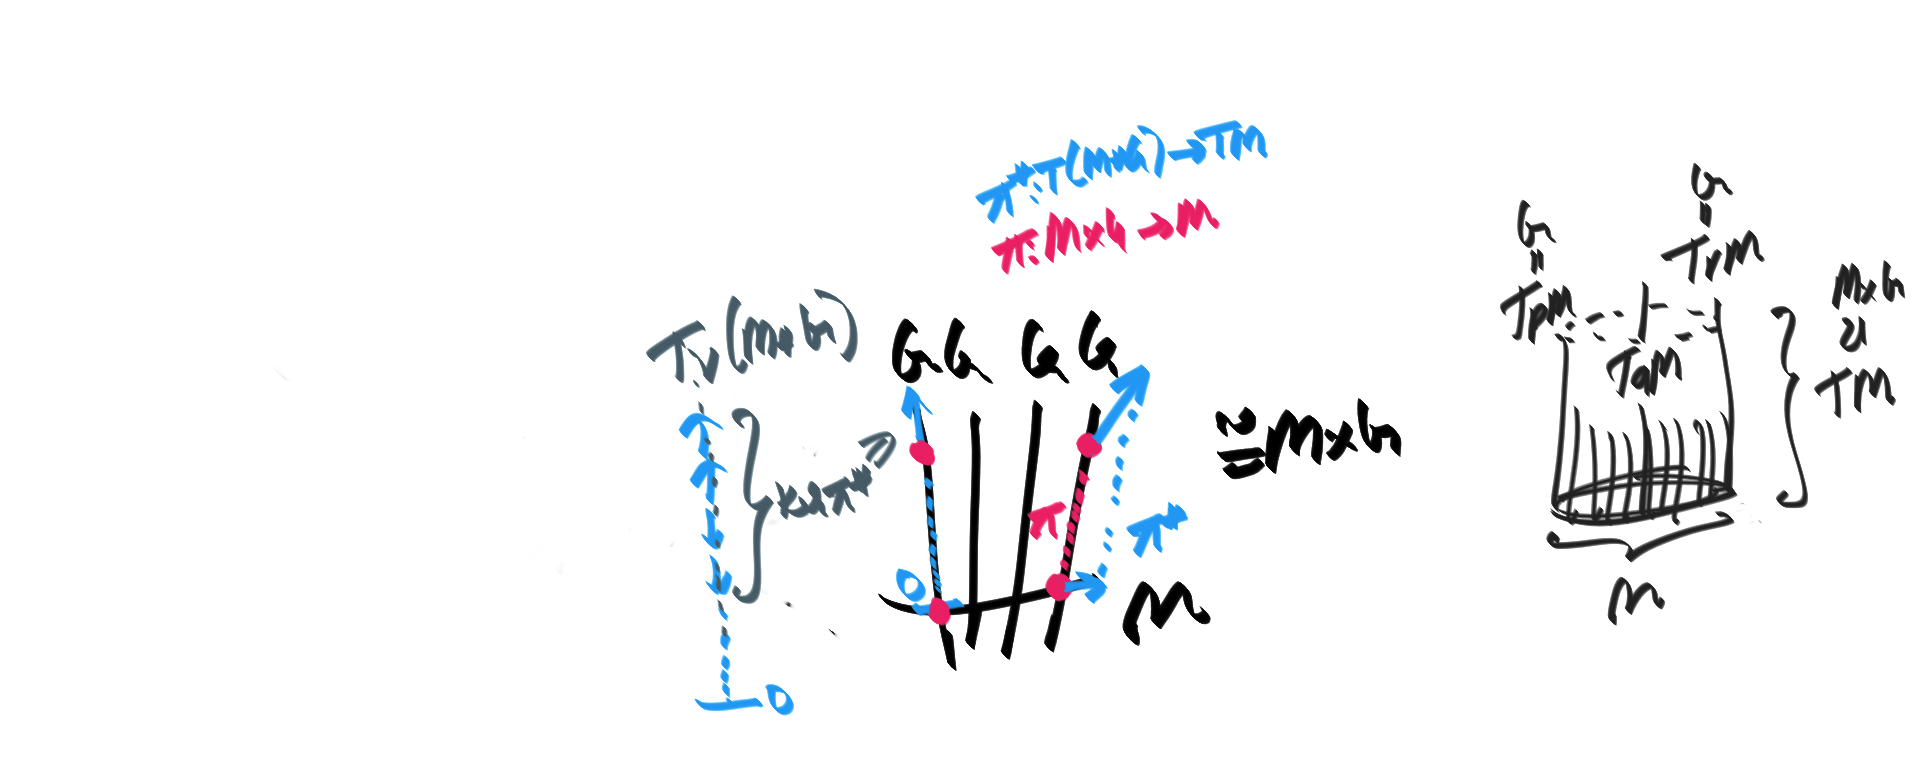
\includegraphics[width=\textwidth]{./g-bundle-pushforward.png}
Pictorially, locally we have the group attached at each point. The projection map 
takes a point and projects it down to the basepoint. The pushforward takes a vector "upstairs"
and pushes it "down" (like what the levi cevita connection does). One way to think
about this is to think about the curve to which the vector is tangent. And then
push forward the curve itself by $\pi$. Then the pushforward of the tangent
is the tangent to the curve that has been pushed forward.
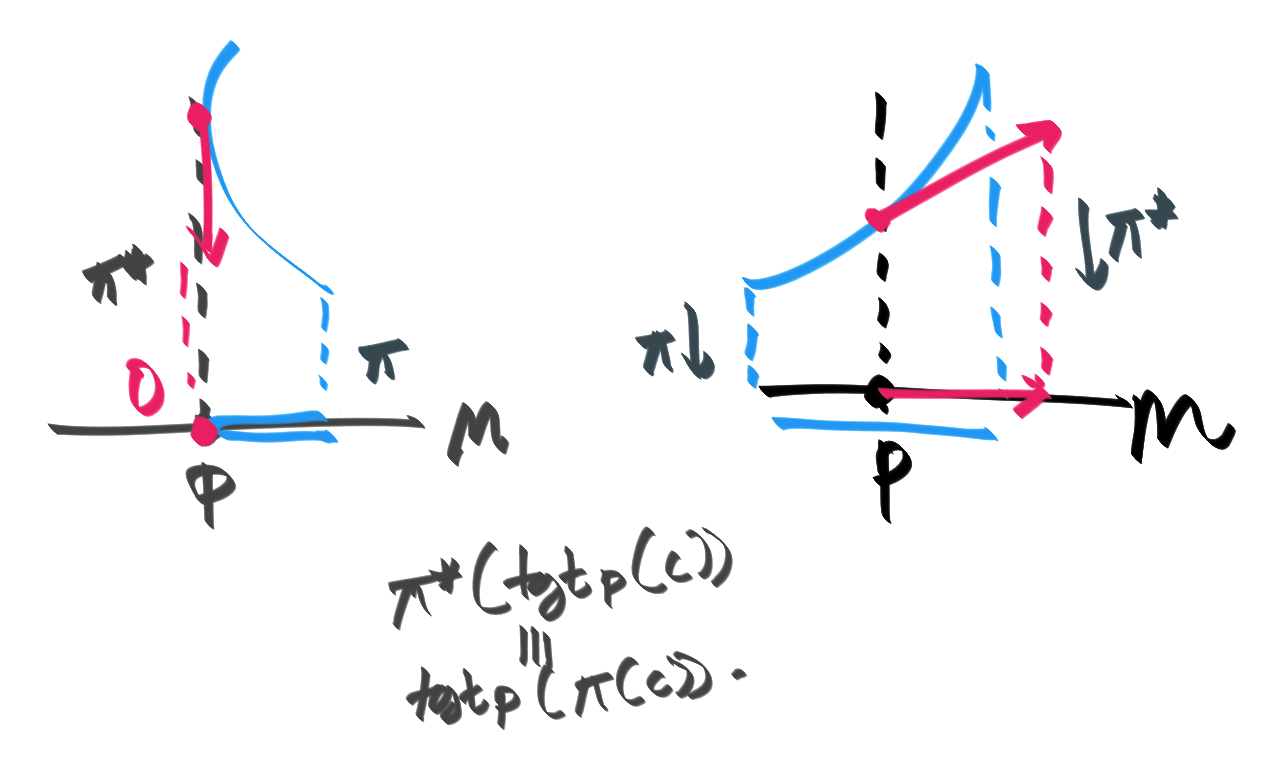
\includegraphics[width=\textwidth]{./g-bundle-pushforward-curves.png}

\begin{lemma}
  For every $p \in P$, the $X^A_p$ lies in the vertical subspace $V_p P$.
  The idea is that the curve that it is defined by, $c^p_a(t) \equiv p \triangleleft \exp (tA)$ lies entirely
  within a fiber due to the action of $\triangleleft$, and thus has zero projection downwards. This is like
  having a curve that is ``vertical'', and thus projects down into the zero curve.
\end{lemma}

\begin{proof}
  The curve lies entirely in the fiber $\pi^{-1}(\pi(p))$. This the projected vector becomes $\pi(c^p_a(t)) = p$.
  This means that $\pi^\star(c^p_a(t)) = \frac{d(\pi(c^p_a(t)))}{dt}|_{dt = 0} = \frac{dp}{dt}|_{t = 0} = 0$.
\end{proof}
\begin{figure}[h]
  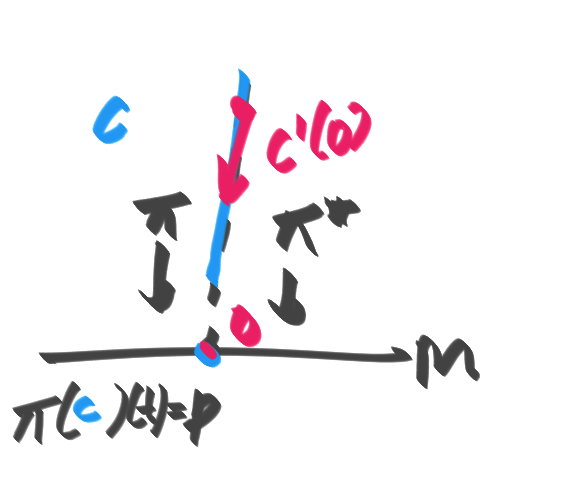
\includegraphics[width=0.5\textwidth]{./g-bundle-pushforward-vertical.png}
  \caption{A curve that lies entirely in a fiber and its  zero pushforward tangent.}
\end{figure}

\begin{definition}
  Connection tells us how to connect neighbouring fibers in the principal bundle.
  To formalize nearby, we need a linearization. We have $V_p P$. Then we make a choice
  of another subspace $H_p P$ such that $V_p P \oplus H_p P$ span the vector space $V$.
  Precisely, a connection on a principal $G$ bundle $P \xrightarrow{\pi} M$ is a
  \emph{distribution} (in the diffgeo sense), ie, an assignment where for each $p \in P$,
  we assign a vector subspace $H_p P \subseteq V_p P$ is chosen such that:
  (1) $H_P \oplus V_p P = T_p P$,
  (2) It's compatible with the $G$ action \emph{within} fibers.
      The push-forward of $H_p P$ by the right action of any $g \in G$ should be compatible
  with the assignment. Formally, $(\triangleleft g)_* (H_p P) = H_{p \triangleleft g} P$.
  (3) It's smooth \emph{across} fibers. The decomposition of any vector $X_p \in T_p P$
  into the horizontal and vertical parts $X_p \equiv hor(X_p) + ver(X_p)$ where $hor(X_p) \in H_p P$,
  and $ver(X_p) \in V_p P$ is unique, and decomposes every smooth vector field $X \in \Gamma(P)$
  into $Hor(X) \in \Gamma(P)$ and $Ver(X) \in \Gamma(P)$  such that $X = Hor(X) + Ver(X)$ and
  these vector fields $Hor(X), Ver(X)$ are smooth. This ensures that the hoizontal components vary
  smoothly across fibers.
\end{definition}

\begin{figure}[h]
  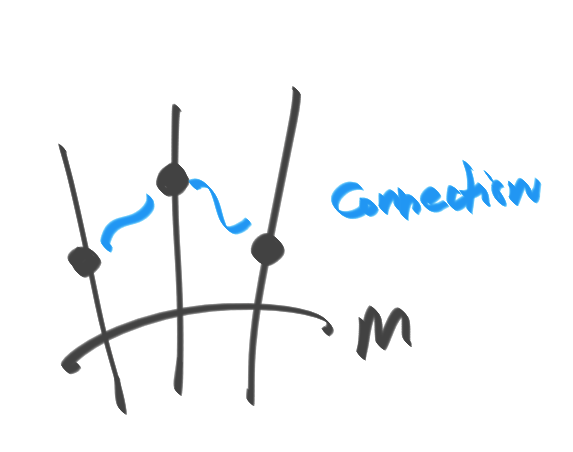
\includegraphics[width=0.3\textwidth]{./connection.png}
  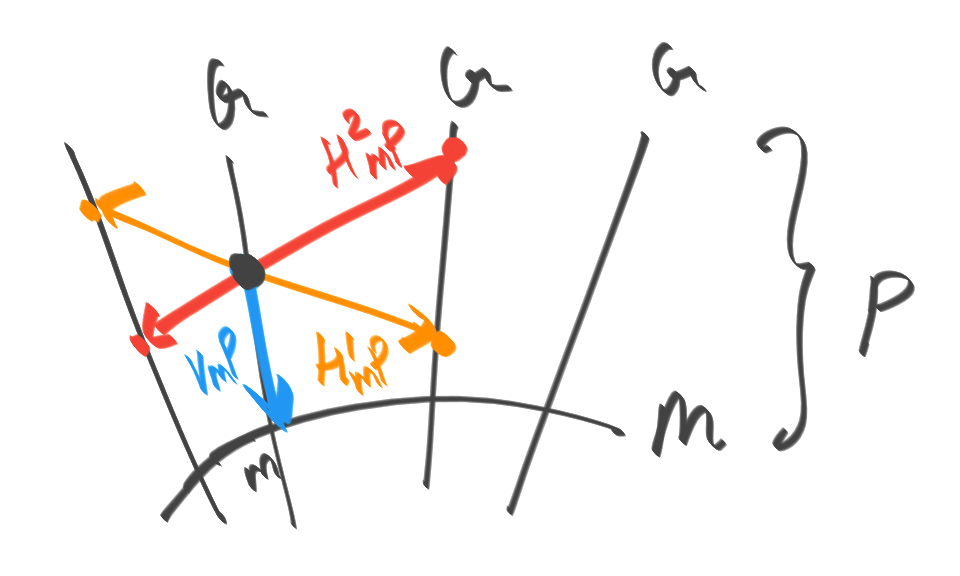
\includegraphics[width=0.5\textwidth]{./connection-hp.png}
  \caption{The idea of a connection, that attempts to connect adjacent spaces. Formally, we try to pick a subspace $H$
  which linearizes the notion of  ``direction of connected point''. }
\end{figure}

\begin{figure}[h]
  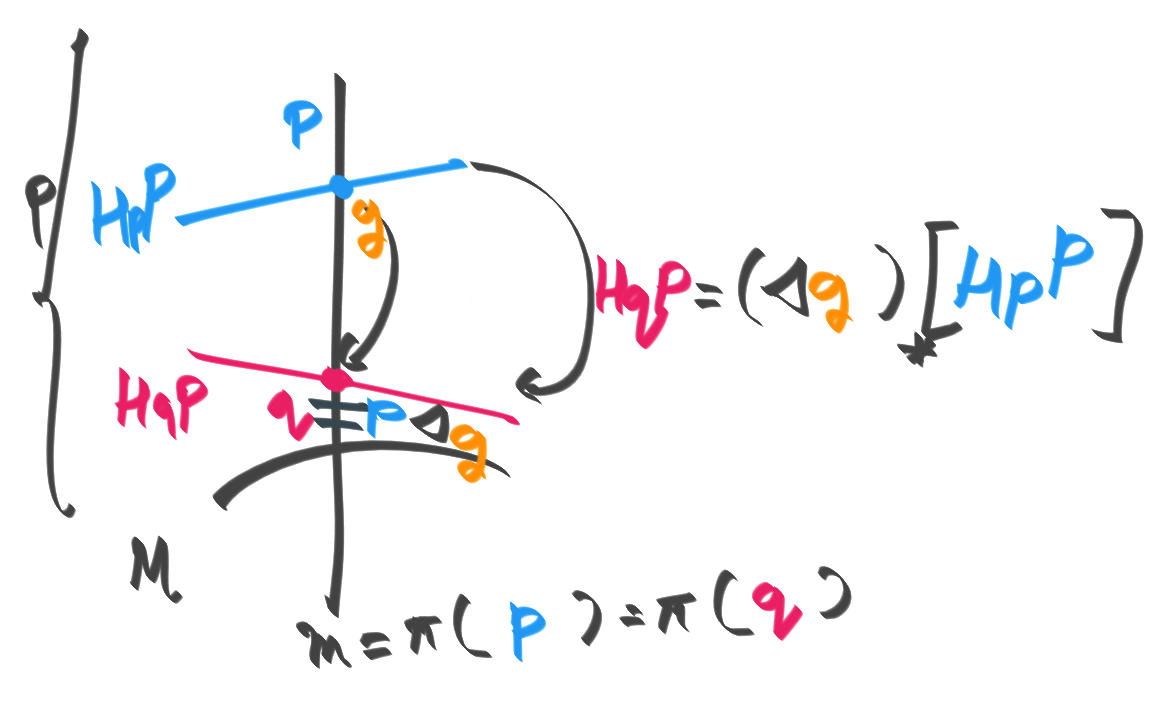
\includegraphics[width=0.5\textwidth]{./connection-condition-in-fiber.png}
  \caption{The connection should be compatible with the group action within fibers}
\end{figure}

\subsection{A caveat of the definition}
The vertical part and the horizontal part $ver(\cdot), hor(\cdot)$ depend on the choice of the $H_p P$.
This is because we cannot ask for the decomposition to be \emph{orthogonal}
Recall that $V_p P$ is given canonically as the kernel of pushforward the projection map.


\begin{figure}[h]
  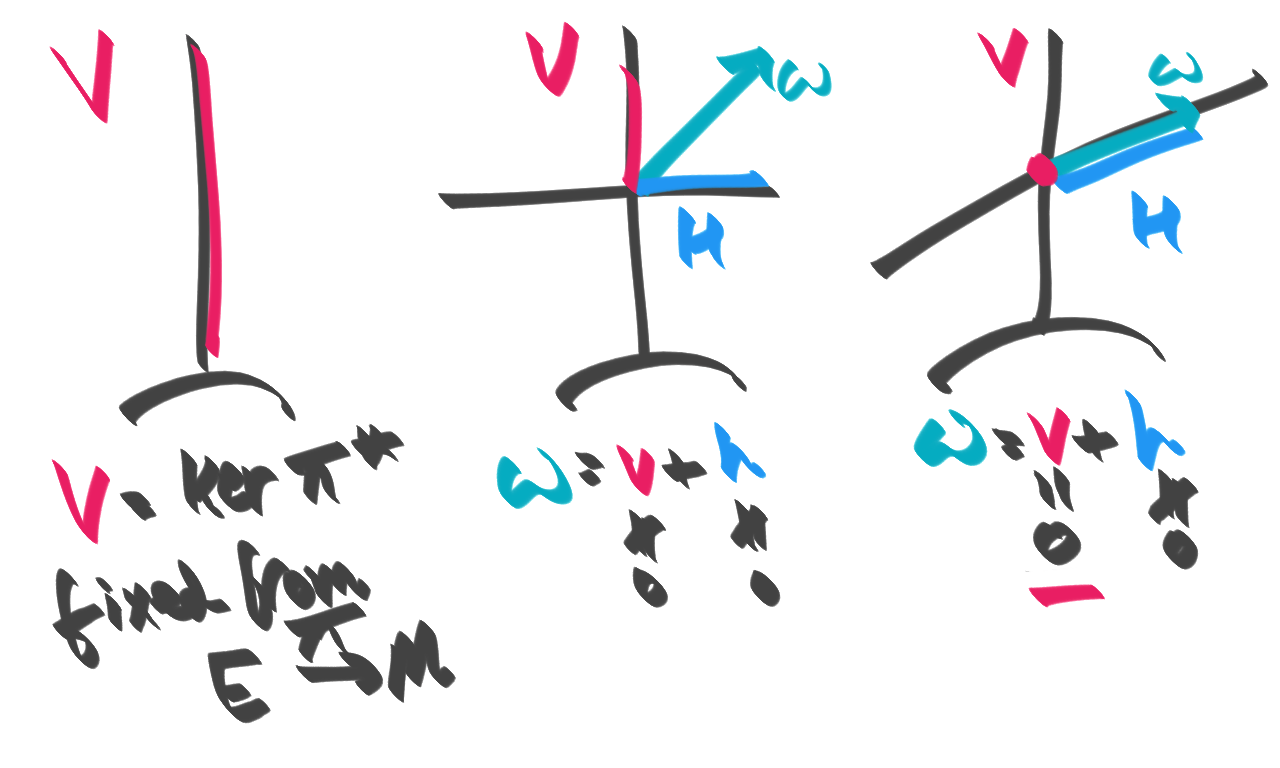
\includegraphics[width=0.8\textwidth]{./connection-ver-depends-on-hor.png}
  \caption{The value of $ver(w) = v$ depends also on the choice of the vector field $H$, since we do not need
    to choose an orthogonal system $V \oplus H$, just a full rank decomposition. This allows us to vary
    $h = hor(w)$ to decrease or increase the component contributed by  $v = ver(w)$.}
\end{figure}

\subsection{Technical definition of choosing horizontal subspace}
Technically, to choose the horizontal subspace $H_p P$ for each $p \in P$ is conveniently encoded
in a lie algebra valued one-form $\omega: TP \rightarrow \mathfrak g$ given by:

\begin{align*}
  &\omega(x_p) \equiv i^{-1}(ver(x_p)) \\
  &i: \mathfrak g = T_e G \rightarrow V_p P \\
  &i: a \mapsto X^a
\end{align*}

So it goes back from the ``left invariant vector field'' $V_p P$ which is determined by a single
lie algebra value $a$, and spits out this lie algebra value. We know that just
looking at $ver (x_p)$ is good enough to give us information about $hor(x_p)$.
This is callect as the connection one-form with respect to the connection given
by the vertical projection $ver_p \equiv  \equiv I - hor_p \equiv I - \pi(H_PP)$,
where $\pi(H_PP)$ is the projector onto the horizontal subspace $H_p P$
See that we can recover the horizontal subspace as $ker(ver_p)$:

\begin{align*}
  &ker(ver_p) \equiv \{ x \in T_p P: ver_p(x) = 0 \} \\
  & = \{  x \in T_pP: (I - hor_p) x = 0 \} \\
  & = \{  x \in T_pP: (x - hor_p(x)  = 0 \} \\
  & = \{  x \in T_pP: (x - \pi(H_p P)(x)  = 0 \} \\
  & = \{  x \in T_pP: x = \pi(H_p P)(x)  \} \\
  & = \{  x \in T_pP: x \in H_p P  \} \\
  ker(ver_p) = H_p P
\end{align*}


We now want to find out what conditions are imposed on $\omega$ from the conditions we had for $H_p P$. Then we
will elevate this to a definition of a connection, such that we can recover an appropriate $H_p P$ from a given
$\omega$.

\begin{theorem}
  A connection one form $\omega$ given by a connection has the following properties:
  (1) $\omega_p(X^a) \equiv a$. This encodes the $i^{-1}$ term we had.

  % https://q.uiver.app/?q=WzAsOSxbMCwwLCJUX2VHIl0sWzIsMCwiKEkgXFxyaWdodGFycm93IEcpIl0sWzQsMCwiKEkgXFxyaWdodGFycm93IFApX3EiXSxbMywwXSxbNiwwLCJUX3FHIl0sWzYsMiwiVF9lRyJdLFs3LDBdLFs1LDFdLFs1LDBdLFswLDEsImkoYSkgXFxlcXVpdiBcXGxhbWJkYSB0LlxcZXhwKHRhKSJdLFsxLDIsImcodCkgXFxtYXBzdG9cXGxhbWJkYSB0LiBxIFxcdHJpYW5nbGVsZWZ0IGcodCkiXSxbMiw0LCJjX3EodCkgXFxtYXBzdG9cXGxhbWJkYSBmLiBcXGZyYWN7ZCAoZlxcY2lyYyBjX3EpfXtkdH1cXGJpZ3xfMCAiLDJdLFs0LDUsImEgXFxtYXBzdG8gaV57LTF9KHZlcihhKSkiXSxbMCw1LCJpZCIsMl1d
\[\begin{tikzcd}
	{T_eG} && {(I \rightarrow G)} & {} & {(I \rightarrow P)_q} & {} & {T_qG} & {} \\
	&&&&& {} \\
	&&&&&& {T_eG}
	\arrow["{i(a) \equiv \lambda t.\exp(ta)}", from=1-1, to=1-3]
	\arrow["{g(t) \mapsto\lambda t. q \triangleleft g(t)}", from=1-3, to=1-5]
	\arrow["{c_q(t) \mapsto\lambda f. \frac{d (f\circ c_q)}{dt}\big|_0 }"', from=1-5, to=1-7]
	\arrow["{a \mapsto i^{-1}(ver(a))}", from=1-7, to=3-7]
	\arrow["id"', from=1-1, to=3-7]
      \end{tikzcd}\]
    
  (2) $((\triangleleft g)^* \omega )_p(x_p) = (Ad_{g^{-1}})_* (\omega_p (x_p) \in T_e G$. Recall that $Ad_g: G \rightarrow G$
  by mapping $Ad_g(h) = ghg^{-1}$. This means that $(Ad_g)_*$ took us from $T_e G$ to $T_{heh^{-1}} G = T_e G$.
    So we have $(Ad_g)_*: T_e \rightarrow T_e$ is a linearization of the conjugation.
  (2) $\omega$ is a smooth one-form. These correspond to (1), (2), (3) of the horizontal subspace definition.
\end{theorem}
\begin{proof}
  (1) is true by the definition of $\omega$. $\omega(X^a) \equiv i^{-1}(ver(X^a))$. But $X^a$ always lies
  in the vertical subspace. so this is $i^{-1}(X^a) = a$, since $i$ maps $a$ to $X^a$.

  
  (2) First observe that the LHS is linear in $X$ as the pullback is a linear function. So we prove it for
  horizontal and vertical part. (2a) Let $x_p \in V_p P$. Then there exists an $a \in \mathfrak g$ such that $x_p = X^a_p$.
  TODO: problem sheet! (Video time: 55:00 --- Conncections and connection 1-forms - Lec 21 - Frederic Schuller)
\end{proof}

\chapter{Lec 22: Local representations of a connection on the base manifold / Yang-Mills fields: Chapter 5.5}

Today, we will study how this lie algebra valued one form on the principal bundle can be locally
writted as a lie algebra valued one form on the base manifold. These are connection coefficients $\Gamma$,
or the Yang-Mills field.

In the last lecture, we considered a principal $G$-bundle $P \xleftarrow{\triangleleft G} P \xrightarrow{\pi} M$.
We had an object that was a lie algebra valued one form:
$\omega: \Gamma(P) \rightarrow \mathfrak g \simeq T_e G$. It had two conditions:
(1) $\omega(X^a) = a$, and (2) $((\triangleleft g)^* \omega)(x) = Ad_{g^{-1}}*(\omega(X))$.

Assume we have a map $u: P \rightarrow P$, a principal bundle automorphism. If we have a one form
that lives $\omega$, if it is a one-form, we should be able to pullback $\omega$ by $u$; Can we still
do so? Do things like pullbacks generalize correctly? The point is that $(u^* \omega(X)) \equiv \omega(u_* X)$.
This works out, because the pullback $u^*$ doesn't actually interact with the $\omega$ at all, it simply  pushes
elements of the domain around. Thus the machinery developed so far continues working!.

In practice, for eg. calculation, one wishes to restrict attention to some subset $U \subseteq M$. Physics
very often starts at a local patch, after which we globalize. Choose a local sectin $\sigma: U \rightarrow P$
such that $\pi(\sigma(u)) = u$. This local section induces two things:

% https://q.uiver.app/?q=WzAsMTIsWzIsMSwiUCJdLFsyLDIsIlUiXSxbMCwyLCJVIl0sWzAsMSwiVSBcXHRpbWVzIEciXSxbMiwwLCJQIl0sWzAsMCwiVSBcXHRpbWVzIEciXSxbNCwxLCJcXEdhbW1hIChUUCkiXSxbNSwxLCJcXG1hdGhmcmFrIGciXSxbMywxLCJcXEdhbW1hKFQoVSBcXHRpbWVzIEcpKSJdLFs0LDIsIlxcR2FtbWEoVFUpIl0sWzUsMl0sWzMsMiwiXFxHYW1tYShUVSBcXG9wbHVzIFRHKSJdLFswLDEsIlxccGkiLDAseyJzdHlsZSI6eyJoZWFkIjp7Im5hbWUiOiJlcGkifX19XSxbMiwxLCJpZCIsMix7InN0eWxlIjp7InRhaWwiOnsibmFtZSI6Imhvb2siLCJzaWRlIjoidG9wIn19fV0sWzMsMiwiZnN0IiwyLHsic3R5bGUiOnsiaGVhZCI6eyJuYW1lIjoiZXBpIn19fV0sWzMsMCwiaCh1LCBnKSBcXGVxdWl2IFxcc2lnbWEodSkgXFx0cmlhbmdsZWxlZnQgZyJdLFswLDQsIlxcdHJpYW5nbGVsZWZ0IEciLDJdLFs2LDcsIlxcb21lZ2EiXSxbOCw2LCJoIl0sWzgsNywiIGheKiBcXG9tZWdhIFxcZXF1aXZcXG9tZWdhIFxcY2lyYyBoIiwwLHsiY3VydmUiOi00LCJzdHlsZSI6eyJib2R5Ijp7Im5hbWUiOiJkYXNoZWQifX19XSxbNiw5LCJcXHBpIiwwLHsic3R5bGUiOnsiaGVhZCI6eyJuYW1lIjoiZXBpIn19fV0sWzksNiwiXFxzaWdtYSIsMCx7ImN1cnZlIjotMX1dLFs5LDcsIlxcb21lZ2FedSBcXGVxdWl2XFxzaWdtYV8qXFxvbWVnYSIsMix7InN0eWxlIjp7ImJvZHkiOnsibmFtZSI6ImRhc2hlZCJ9fX1dLFs1LDQsImgiXSxbMSwwLCJcXHNpZ21hIiwyLHsiY3VydmUiOjJ9XSxbMyw1LCJcXHRyaWFuZ2xlbGVmdCBHIiwwLHsibGFiZWxfcG9zaXRpb24iOjQwfV0sWzgsMTFdLFsxMSw4LCJcXHNpbWVxIl1d
\[\begin{tikzcd}
	{U \times G} && P \\
	{U \times G} && P & {\Gamma(T(U \times G))} & {\Gamma (TP)} & {\mathfrak g} \\
	U && U & {\Gamma(TU \oplus TG)} & {\Gamma(TU)} & {}
	\arrow["\pi", two heads, from=2-3, to=3-3]
	\arrow["id"', hook, from=3-1, to=3-3]
	\arrow["fst"', two heads, from=2-1, to=3-1]
	\arrow["{h(u, g) \equiv \sigma(u) \triangleleft g}", from=2-1, to=2-3]
	\arrow["{\triangleleft G}"', from=2-3, to=1-3]
	\arrow["\omega", from=2-5, to=2-6]
	\arrow["h", from=2-4, to=2-5]
	\arrow["{ h^* \omega \equiv\omega \circ h}", curve={height=-24pt}, dashed, from=2-4, to=2-6]
	\arrow["\pi", two heads, from=2-5, to=3-5]
	\arrow["\sigma", curve={height=-6pt}, from=3-5, to=2-5]
	\arrow["{\omega^u \equiv\sigma_*\omega}"', dashed, from=3-5, to=2-6]
	\arrow["h", from=1-1, to=1-3]
	\arrow["\sigma"', curve={height=12pt}, from=3-3, to=2-3]
	\arrow["{\triangleleft G}"{pos=0.4}, from=2-1, to=1-1]
	\arrow[from=2-4, to=3-4]
	\arrow["\simeq", from=3-4, to=2-4]
      \end{tikzcd}\]
    
    
\begin{itemize}
\item  A \emph{Yang-Mills field} $\omega^U: \Gamma(TU) \rightarrow T_e G$. See that we now get a lie algebra valued
one-form  over the
\emph{base manifold} $\Gamma(U)$, not over $\Gamma(P)$. This is given by $\omega^u \equiv \sigma^* \omega$.
That is, $\omega^U(v_u \in T_u M) \equiv \omega(\sigma_*(v_u))$ where $\sigma_*: TU_p \rightarrow TP_{\sigma(p)}$
  is the jacobian of $\sigma$.

\item This section can be used to define a local trivialization of the principal bundle.  This is $h: U \times G \rightarrow P$.
  This is defined as $h(u, g) \equiv \sigma(u) \triangleleft g$ $\sigma$ moves into $P$, and then $g$ slides along the fiber.
  One we have this local trivialization, we can define the local representation of the connection one-form as the pullback of
  $\omega$ along $h$ --- $h^* \omega$.
\end{itemize}

\begin{theorem}
  $(h^*\omega)(v \in T_m U, \gamma \in T_g G) = Ad_{g^{-1}}*(\omega^u(v)) + \Xi_g(\gamma)$.

  See that the $Ad_{g^{-1}}: T_g G \rightarrow T_eG$. So this extra addition $Xi_g: T_g G \rightarrow T_e G$. We can
  understand the values in the tangent vector space  $T_g G$ as the value of a left-invariant vector field
  generated by a lie algebra element. So this spits out the lie algebra element that generates this lie group element.
  This map is called the \emph{Maurer-Cartan form} on the lie group $G$. It is a lie algebra
  valued on form on the lie group $G$.. Intuitively, given a $\gamma \in T_g G$,
  it creates the left-invariant vector field $L(\gamma)$ that has value $\gamma$ at $g$:
  $L(\gamma)(g) = g$. It then evaluates $L(\gamma)(e) \in T_e G$ to find the correct lie algebra element
  $L(\gamma)(e) \in  \mathfrak g$. This $Xi$ is fixed; it's a property of the group. 
\end{theorem}

\begin{example}
  Example for motivation to choose particular section $\sigma: U \rightarrow P$.
  Consider an $n$-dimensional manifold and the frame bundle
  as an example, $P \equiv LM$. Any chart $(U, \phi: U \rightarrow \mathbb R^n)$ of the base manifold $M$ induces a section!
  $\sigma(m \in U) = (\frac{d\phi}{dx^1}|_m, \dots, \frac{d\phi}{dx^n}|_m) \in GL_n(\mathbb R)$.
  At each point, we have a basis induced by $\phi$. That's the section of the frame bundle.

  Then the Yang-mills field, $\omega^U \equiv \sigma^*\omega$ is a one-form on $U$ that is lie-algbera
  valued. The lie algebra of $G \equiv GL(n, \mathbb R)$ is $M_n(\mathbb R)$, all matrices. This means
  it has type $\omega^U: \Gamma(TU) \rightarrow M_n(\mathbb R)$. So at a point, it has the type
  $\omega^U_p: T_p U \rightarrow M_n(\mathbb R)$. So it needs components lower-$\mu$ to consume a $T_p$,
  and then a lower and upper $i, j$ to represent $M_n$. This means we have the coordinate values
  $\Gamma^i_{j, \mu}$ in local coordinates. But the $i, j$ label the lie algebra, while $\mu$ actually
  has something to do with the base manifold. That's why it doesn't transform as a tensor!
  These are the Christoffel coefficients.
\end{example}

\begin{example}
  Construction of the Mauer Cartan form $\Xi$ for the lie group $G$ given by $GL(d, \mathbb R)$.
  Choose coordinates on an open set $G^+$ of $G$ containing the identity $e \in G$.
  Now consider $L^A_g$, a left invariant vector field. This can be applied to coordinate functions.
  So we evaluate $L^A_g(x^i_j) = \frac{d (x^{i}_j \circ [g \cdot exp(tA)])}{dt}|_0$.
  If we consider everything in terms of coordinates, then we replace $exp$ with the matrix
  exponential: $L^A_g = \frac{d (x^{i}_j \circ [g \cdot e^{tA}])}{dt}|_0$. But $x^i_j$ is the
  thing that pulls out matrix entries. So let's write $g$ also as matrix entries. This becomes:

  
% \begin{align*}
% &\frac{d {x^i_j(g^p_k (e^{tA})^k_r)}}{dt}|_0 \\
% &\frac{d {\delta^i_p \delta_j^r g^p_k (e^{tA})^k_r}}{dt}|_0 \\
% &\frac{d {g^i_k e^{tA})^k_j}{dt}|_0 \\
% &\frac{d {g^i_k (I + tA + \dots))^k_j}{dt}|_0 \\
% &g^i_kA^k_j
% \end{align*}

So therefore $L^A_g = g^i_k A^k_j \frac{\partial}{\partial x^i_j}$. This is a basis of the tangent space.
WTF, this would have been so much easier if we had just calculated at identity and then pushed forward.
The Mauer cartan form $Xi_g: T_g G \rightarrow T_e G$. Here, we simply need to invert.
So we get $\Xi_{@g, j}^i \equiv (g^{-1})^i_k (dx^k_j)$. Compare:
% \begin{align*}
% &L^A_g  \equiv g^i_k \cdot A^k_j \cdot \frac{\partial}{\partial x^i_j} \\
% &\Xi_{@g} \equiv g^{-1}^i_k \cdot I \cdot dx^k_j \\
% &\Xi_{@g}(L^A_g) = g^{-1}^i_k (dx^k_j) (g^p_r A^r_q \frac{\partial}{\partial x}^p_q) \\
% & = A^r_q \cdot g^{-1}^i_k g^p_r  [dx^k_j  \frac{\partial}{\partial x}^p_q] \\
% & = A^r_q \cdot g^{-1}^i_k g^p_r delta^k_q \delta_j^p  \\
% & = A^r_q \cdot g^{-1}^i_q g^p_r  \delta_j^p  \\
% &= 
% &= A^i_j
% x\end{align*}

(55:54) TODO: continue watching lecture
\end{example}

\chapter{Parallel transport: Lecture 23}
\url{https://www.youtube.com/watch?v=jGHaZc2fuX8&list=PLPH7f_7ZlzxTi6kS4vCmv4ZKm9u8g5yic&index=23}.

The basic idea: $P \xrightarrow{\pi} M$ with group $G$. Let the dimension of $G$ be one, and the dimension
of $M$ be 2. If $G$ has a connection 1-form $\omega$, which defines at each point $H_p P$.

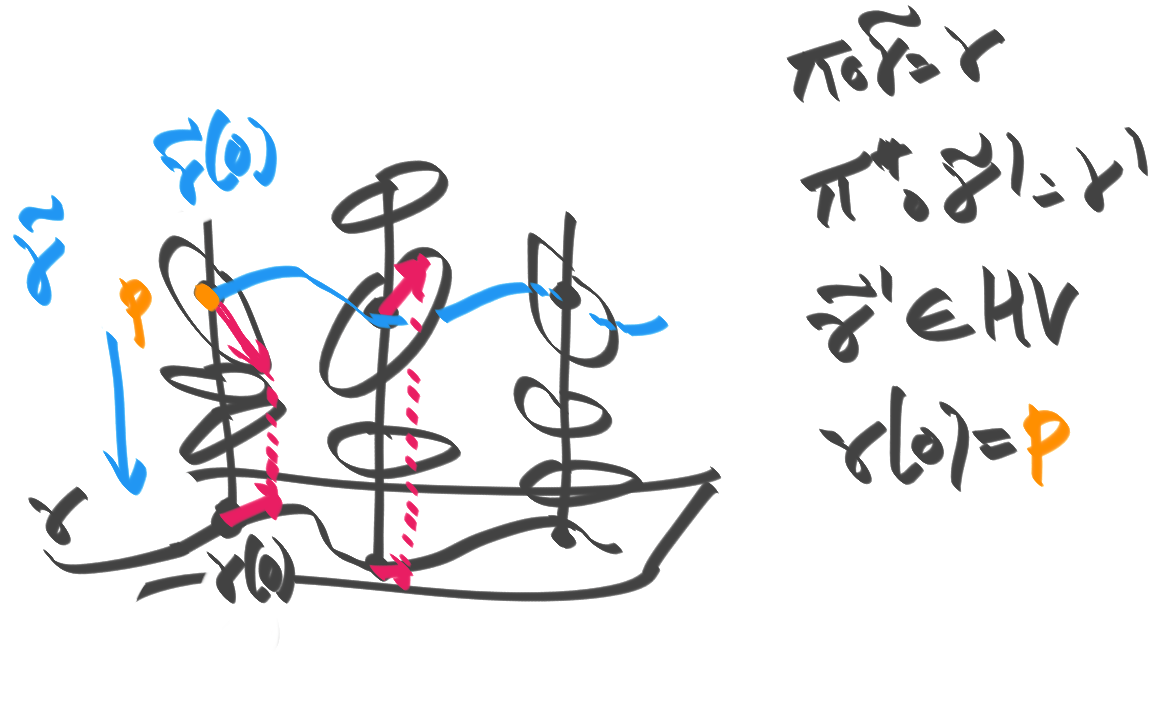
\includegraphics[width=\textwidth]{./parallel-transport.png}

\chapter{5.7: Curvature and torsion on principal bundles}

Torsion requires additional structure beyond what a principal bundle has.
The usual linear covariant derivative carries a frame bundle.

\begin{definition}
  If we have $P \xleftarrow{\triangleleft G} P \xrightarrow{\pi} M$ with a connection $\omega$,
  and let $\phi$ be a $\FiveFlowerPetal$ (arbitrary)
  valued $k$-form, then $D(\phi): \Gamma(T^{k+1} P) \rightarrow \FiveFlowerPetal$. It is defined as the ordinary
  exterior derivative (which does not depend on $\FiveFlowerPetal$ at all) given by:

  $$
  D\phi(X_1, \dots, X_{k+1}) \equiv d \phi(hor(X_1), hor(X_2), \dots, hor(X_{k+1}))
  $$

  We need $\omega$ to define $hor$. This is the covariant exterior derivative of the $k$ form $\phi$.
\end{definition}

\begin{definition}
  Curvature: We once again have $P \rightarrow M$ and a one-form $\omega: \Gamma(TP) \rightarrow \mathfrak g$.
  Then the curvature of the connection is a lie-algebra valued two-form $\Omega: \Gamma(T^2P) \rightarrow \mathfrak g = T_e G$
  defined as $\Omega \equiv d\omega$.

\end{definition}

We claim that $d\Omega = d\omega + \omega \barwedge \omega$.
See that we use a special $\barwedge$. We know that the usual exterior derivative is antisymmetric,
and thus $\omega \wedge \omega = 0$. But here, since we live in lie-groups, we get non-commutativity,
and hence $\omega \barwedge \omega$ need not disappear! We define this as:

$$
(\omega \barwedge \omega)(X \in \Gamma(TP), Y \in \Gamma(TP)) \equiv [\omega(X) , \omega(Y)]
$$

If the lie group is a matrix group, then we can write $\Omega^i_j \equiv d \omega^i_j + \omega^i_k \wedge \omega^k_j$.
The wedge is sort of like a commutator.


\begin{proof}
  We know that $\omega$ is bilinear. Decompose any vector into a vertical and horizontal part, and then
  prove separately. TODO: (time: 16:02).
\end{proof}

\section{Relation to the base space}

How do these definitions relate to objects on the base space? We have $\omega$ and $\Omega$ on the
principal bundle $P$. We have some section $\sigma: U \rightarrow P$ of $\pi: P \rightarrow M$.
This induces a Yang-mills field  $\Gamma \equiv \sigma^* \omega$ which is a lie algebra valued one form
on the base space. This also introduces a Yang-mills field strength ($F$). The field is $A$, the vector potential.
This Yang-Mills field strength is the pullback of the curvature. This is $\sigma^* Omega \simeq Riem \simeq F$.
(Riem for Riemann curvature tensor, I guess). They live in $TM \otimes TM \rightarrow \mathfrak g$. Why is this
well behaved (a tensor) while the christoffel symbols are not?

\begin{align*}
  \sigma^*(\Omega) \\
  & = \sigma^*(d\omega + \omega \barwedge \omega) \\
  &= \sigma^*(d \omega) + \sigma^*(\omega \barwedge \omega) \\
  &\sigma^*\texttt{distributes over } \barwedge \\
  &= \sigma^*(d \omega) + \sigma^*(\omega) \barwedge \sigma^*(\omega) \\
  & \sim \partial \Gamma - (\partial \Gamma \Gamma \Gamma + \Gamma \Gamma) \texttt{(wut?)} \\
\end{align*}

\begin{theorem}
  Binanchi identity for curvature: $D \Omega = 0$. Recall that $\Omega = D \omega$.
  This is NOT because $D^2 = 0$, $D^2 \neq 0$ in general, it's not homological.
  Proof on problem sheet.
\end{theorem}

\section{Torsion}
We have a connection one form $\omega_p: T_pP \rightarrow \mathfrak g$ on a principal $G$ bundle $P \xrightarrow{x} M$.
We need some extra data $\theta_p: T_p P \rightarrow V$ --- it is a $V$ valued one-form on $P$, is called a
\emph{solder form / soldering form}. Here, $V$ is a linear representation
of the group $G$ with the same dimension as that of the base manifold. The precise conditions are:

\begin{itemize}
  \item $\Theta \in \Omega^1(P) \otimes V$, where $V$ is a linear representation of the group $G$
  \item $dim(V) = dim(M)$.
  \item $\Theta$ is a vertical form:  We have $\Theta(ver(X)) = 0$ for all vector fields $X \in \Gamma(TP)$.
    So this is a vertical one-form. This is unlike the the connection one-form which vanishes on the horizontal vector field,
    which is why we can recover the horizontal direction as the kernel.
  \item $g \triangleright ((\triangleleft g)^*\Theta) = \Theta$ ($G$-equivariance)
  \item $TM \simeq P_V$. The tangent bundle of the base manifold is supposed to be isomorphic to the associated bundle
      associated to $P$. We need them to be the same as associated bundle maps.
    \end{itemize}

\subsection{Idea}
The soldering form is introduced to provide an identification of this chosen vector space $V$ with each
tangent space of $M$. The key example is as usual, the frame bundle. We define the $\Theta$ as a one form
$\Theta: \Gamma(TP) \rightarrow \mathbb R^{dim M} \simeq V$. We define this for each frame  $e \in P$.
$\Theta_e(X) \equiv u_e^{-1}(\pi_*(x)))$
Where $u_e: \mathbb R^{dim M} \rightarrow T_{\pi e} M$ by $u_e(v) = ev$.

We know that if there is a frame $e$, there is a coframe $\epsilon$.
I'm lost! Time: around 1 hour into video

\begin{definition}
  Torsion is the exterior derivative of the solder form. $\Theta \equiv d \theta$ which is $\Theta \in \Omega^2(P) \otimes V$.
  One can see that $\Theta = d \theta + \omega \wedge \theta$. In diffgeo, we have to identify the
  torsion with the coframe. For a matrix group, we get $\Theta^i =  d \theta^i  + \omega^i_k \wedge \theta^k$.
\end{definition}

\begin{theorem}
  Bianchi identity of torsion: $D \Theta = \Omega \barwedge \theta$.
\end{theorem}

\chapter{5.8: Lecture 25: Covariant derivatives}

We can ask that the associate bundle is a vector space $F$, and that the
left action of $G$ on the associated bundle to be linear. Then we can
do the usual rigamarole of parallel transport, etc. to write down the covariant
derivative.
\begin{quote}
  It is very geometric, it is very intuitive, and it is technically a disaster
\end{quote}

\section{Technically neater construction}

Once again, we need $F$ a vector space and a linear left action.  For a given
$\sigma: M \rightarrow P$ we define an associate function $\phi_\sigma: P \rightarrow F$
Then we need this $\phi_\sigma$ to be $G$-equivariant. We then use the exterior covariant
derivative on $P$ to get a derivataive of the function sitting up on the $P$.
Then we need to push this down to the manifold. We work on the principal bundle ONLY.



\end{document}




